%
%  Documentation on Nalu
%
\documentclass[12pt]{report}
\usepackage{ifpdf}
\usepackage{graphicx}
\usepackage{amsmath}
\usepackage{ifthen}         % Conditional switching of mathmodels text
\usepackage{cmap}           % Make ligatures searchable and copyable
\usepackage[T1]{fontenc}
\usepackage{color}
\usepackage{listings}
\ifpdf
  \usepackage[
     pdftitle={Nalu Theory Manual},
     pdfpagemode=UseOutlines,
     pdfstartview=FitH,
     bookmarksopen=false,
     bookmarksnumbered=true,
     colorlinks=true,
     linkcolor=blue,
     citecolor=blue,
     urlcolor=blue
  ]{hyperref}
\fi

% Define this as the theory manual for conditional text within the document
\newcommand{\manual}{theory}

\graphicspath{{./figures/}}  % Figure file location
\topmargin 0.0in      % Top offset from a point 1 inch in from edge
\oddsidemargin 0.0in  % Left offset from a point 1 inch in from edge
\headheight 0.0in     % Height of header block
\headsep 0.0in        % Gap between bottom of header block and top of body
\topskip 0.0in        % Distance from top of body to baseline of first text line
\textwidth 6.5in
\textheight 9.0in

% Define some shorthand notation
\newcommand{\pd}[2]{\frac{\partial{#1}}{\partial{#2}}}
\newcommand{\half}{\frac{1}{2}}
\newcommand{\iph}{{i+\frac{1}{2}}}
\newcommand{\imh}{{i-\frac{1}{2}}}

\begin{document}

\include{widehat}   % Custom hat that can grow to arbitrarily large sizes
\include{widetilde} % Custom tilde that can grow to arbitrarily large sizes

\thispagestyle{empty}

\phantom{.}
\vspace{1.0in}

\noindent
\begin{tabular}{l}
{\Large \bf Sierra Low Mach Module: Nalu} \\
{\Large \bf Theory Manual -- Version 1.0} \\[12pt]
\rule[5pt]{6.5in}{0.05in} \\
\end{tabular}

\vspace{1.5in}

Sandia is a multiprogram laboratory operated by Sandia Corporation, a Lockheed Martin
Company for the United States Department Of Energy's National Nuclear
Security Administration under Contract DE-AC04-94AL85000.

\vspace{3.0in}

\noindent
\begin{tabular}{l}
{\large \bf Sandia National Laboratories} \\
{Albuquerque, New Mexico} \\
{web: \texttt{\href{http://github.com/spdomin/Nalu}{http://github.com/spdomin/Nalu}}} \\
{\large \bf SAND2015-3107W -- Unclassified Unlimited Release, UUR} \\
{\bf \today} \\
\rule[7pt]{6.5in}{0.025in}
\end{tabular}

\clearpage
\pagenumbering{roman}
\setcounter{page}{2}

\clearpage
\tableofcontents

\clearpage
\ifpdf
  \phantomsection\label{listoffigures}
\fi
\addcontentsline{toc}{figure}{List of Figures}
\listoffigures

\clearpage
\ifpdf
  \phantomsection\label{listoftables}
\fi
\addcontentsline{toc}{table}{List of Tables}
\listoftables

\clearpage
\pagenumbering{arabic}
\setcounter{page}{1}

%%%%%%%%%%%%%%%%%%%%%%%%%%%%%%%%%%%%%%%%%%%%%%%%%%%%%%%%%
\section{Introduction}
\input{introduction}

\section{Low Mach Number Derivation}
\input{lowMachNumberDerivation}

\section{Supported Equation Set}
This section provides an overview of the currently supported
equation sets. Equations will be described in integral form with
assumed Favre averaging. However, the laminar counterparts
are supported in the code base and are obtain in the user file
by omitting a turbulence model specification. 

\subsection{Conservation of Mass}
The continuity equation is always solved in the variable density form.

\begin{equation}
\int \frac{\partial \bar{\rho}} {\partial t}\, dV
+ \int \bar{\rho} \tilde{u}_i  n_i\, dS = 0
\end{equation}
Since Nalu uses equal-order interpolation (variables are collocated)
stabilization is required. The stabilization choice will be developed
in the pressure stabilization section.

Note that the use of a low speed compressible formulation requires that 
the fluid density be computed by an equation of state that uses the 
thermodynamic pressure. This thermodynamic pressure can either be computed
based on a global energy/mass balance or allowed to be spatially varying.
By modification of the continuity density time derivative to include 
the $\frac{\partial \rho}{\partial p}$ sensitivity,
an equation that admits acoustic pressure waves is realized.

\subsection{Conservation of Momentum}

The integral form of the Favre-filtered momentum equations used for
turbulent transport are
%
\begin{eqnarray}
   \int {{\partial \bar{\rho} \tilde{u}_i} \over {\partial t}} {\rm d}V
  +  \int \bar{\rho} \tilde{u}_i \tilde{u}_j n_j {\rm d}S 
   &=& 
   \int \tilde{\sigma}_{ij} n_j {\rm d}S 
  - \int \tau^{sgs}_{ij} n_j {\rm d}S \nonumber \\ 
   &+& \int \left(\bar{\rho} - \rho_{\circ} \right) g_i {\rm d}V,
\label{fav-mom}
\end{eqnarray}
%
where the subgrid scale turbulent stress $\tau^{sgs}_{ij}$ is defined as
%
\begin{equation}
\tau^{sgs}_{ij} \equiv \bar{\rho} ( \widetilde{u_i u_j} - 
     \tilde{u}_i \tilde{u}_j ).
\label{sgsStress}
\end{equation}
%
The Cauchy stress is provided by,
\begin{equation}
\sigma_{ij}  = 2 \mu \tilde S^*_{ij} - \bar P \delta_{ij}
\end{equation}
%
and the traceless rate-of-strain tensor defined as follows:
\begin{eqnarray}
\tilde S^*_{ij}  &=& \tilde S_{ij} - \frac{1}{3} \delta_{ij} \tilde S_{kk} \nonumber \\
		     &=& \tilde S_{ij} - \frac{1}{3} \frac{\partial \tilde u_k }{\partial x_k}\delta_{ij}.
\end{eqnarray}

In a low Mach flow, as described in the low Mach theory section, 
the above pressure, $\bar P$ is the perturbation about the thermodynamic
pressure, $P^{th}$. In a low speed compressible flow, i.e., flows confined to a closed
domain with energy or mass addition in which the continuity equation
has been modified to accommodate acoustics, this pressure is interpreted at the
thermodynamic pressure itself.

For LES, $\tau^{sgs}_{ij}$ that appears in Equation~\ref{fav-mom} and defined in 
Equation~\ref{sgsStress} represents the subgrid stress tensor that must be closed.  The deviatoric part of the subgrid stress tensor is defined as,
%
\begin{equation}
\tau^{*sgs}_{ij} = \tau^{sgs}_{ij} - \frac{1}{3} \delta_{ij} \tau^{sgs}_{kk}
\end{equation}
%
where the subgrid turbulent kinetic energy is defined as $\tau^{sgs}_{kk} = 2 \bar \rho k$.
Note that here, k represents the modeled turbulent kinetic energy as is formally defined as,

\begin{equation}
\bar \rho k = \frac{1}{2} \bar\rho ( \widetilde{u_k u_k} - \tilde u_k \tilde u_k).
\end{equation}
%
Model closures can use, Yoshikawa's approach when k is not transported:

\begin{equation}
\tau^{sgs}_{kk} = 2 C_I \bar \rho \Delta^2 | \tilde S | ^2.
\end{equation}
%
Above, $ | \tilde S | = \sqrt {2 \tilde S_{ij} \tilde S_{ij}}$

For low Mach-number flows, a vast majority of the turbulent kinetic energy
is contained at resolved scales. For this reason, the subgrid turbulent kinetic energy is not 
directly treated and, rather, is included in the pressure as an
additional normal stress.  The Favre-filtered momentum equations then become
%
\begin{eqnarray}
\lefteqn{ \int {{\partial \bar{\rho} \tilde{u}_i} \over {\partial t}}
     {\rm d}V + \int \bar{\rho} \tilde{u}_i \tilde{u}_j n_j {\rm d}S 
   + \int \left( \bar{P} + \frac{2}{3} \bar{\rho} k \right) 
     n_i {\rm d}S = } \nonumber \\
   && \int 2 (\mu + \mu_t) \left( \tilde{S}_{ij} - \frac{1}{3}
      \tilde{S}_{kk} \delta_{ij} \right) n_j {\rm d}S
    + \int \left(\bar{\rho} - \rho_{\circ} \right) g_i {\rm d}V,
\label{mod-mom-les}
\end{eqnarray}
%
where LES closure models for the subgrid turbulent eddy viscosity
$\mu_t$ are either the constant coefficient Smagorinsky, WALE or the constant 
coefficient $k_{sgs}$ model (see the turbulence section).

\subsubsection{Earth Coriolis Force}
For simulation of large-scale atmospheric flows, the following Coriolis force
term can be added to the right-hand-side of the momentum equation
(\ref{fav-mom}):
\begin{equation} \label{cor-term}
  \int -2\bar{\rho}\epsilon_{ijk}\Omega_ju_k ~{\rm d}V.
\end{equation}
Here, $\Omega$ is the Earth's angular velocity vector, and
$\epsilon_{ijk}$ is the Levi-Civita symbol denoting the cross product
of the Earth's angular velocity with the local fluid velocity
vector. Consider an ``East-North-Up'' coordinate system on the Earth's
surface, with the domain centered on a latitude angle $\phi$ (changes
in latitude within the computational domain are neglected). In this
coordinate system, the integrand of (\ref{cor-term}), or the Coriolis
acceleration vector, is
\begin{equation} \label{cor-acc}
  2 \bar{\rho} \omega
  \begin{bmatrix} u_n \sin\phi - u_u \cos\phi \\
                  -u_e \sin\phi \\
                  u_e \cos\phi
  \end{bmatrix},
\end{equation}
where $\omega \equiv ||\Omega||$.  Often, in geophysical flows it is
assumed that the vertical component of velocity is small and that the
vertical component of the acceleration is small relative to gravity,
such that the terms containing $\cos\phi$ are neglected.  However,
there is evidence that this so-called traditional approximation is not
valid for some mesoscale atmospheric phenomena \cite{Gerkema_etal:08},
and so the full Coriolis term is retained in Nalu.  The implementation
proceeds by first finding the velocity vector in the East-North-Up
coordinate system, then calculating the Coriolis acceleration vector
(\ref{cor-acc}), then transforming this vector back to the model
$x-y-z$ coordinate system.  The coordinate transformations are made
using user-supplied North and East unit vectors given in the model
coordinate system.

\subsubsection{ABL Forcing Source Terms} \label{sec:abl-forcing}

In LES simulations of wind plant atmospheric flows, it is often necessary to
drive the flow a predetermined vertical velocity and/or temperature profile. In
Nalu, this is achieved by adding appropriate source terms $\mathbf{S}_u$ to the
momentum equations (\ref{fav-mom}). The present implementation can vary the
source terms as a function of time and space using either a user-defined table
of previously computed source terms (e.g., from a \emph{precursor} simulation or
another model such as WRF), or compute the source term as a function of the
transient flow solution using the following equation:
\begin{align}
  \label{eq:abl-mom-source}
 \mathbf{S}_u^n &= \alpha_u \bar{\rho} \left( \frac{\mathbf{U}^n_\mathrm{ref} -
                  \left<\mathbf{u}^n\right>}{\Delta t^n}\right)
\end{align}
where $\left<\mathbf{u}^n\right>$ is the horizontally averaged velocity at a
given height and instance in time $t=t_n$, $\mathbf{U}^n_\mathrm{ref}$ are the desired
velocities at the corresponding heights and time. The implementation allows the
user to prescribe relaxation factors $\alpha_u$ for the source terms that are
applied. Nalu uses a default value of $1.0$ for the relaxation factors if no
values are defined in the input file during initialization.

\subsection{Filtered Mixture Fraction} \label{sec:filtered_Z}

The optional quantity used to identify the chemical state is the mixture 
fraction, $Z$.  While there are many 
different definitions of the mixture fraction that have subtle variations
that attempt to capture effects like differential diffusion, they can all 
be interpreted as a local mass fraction of the chemical elements that
originated in the fuel stream.  The mixture fraction is a
conserved scalar that varies between zero in the secondary stream and unity in the
primary stream and is transported in laminar flow by the equation,
%
\begin{equation}
\frac{\partial \rho Z}{\partial t}
  + \frac{ \partial \rho u_j Z }{ \partial x_j}
  = \frac{\partial}{\partial x_j} \left( \rho D \frac{\partial Z}{\partial x_j}
    \right),  \label{eqn:lam_Z}
\end{equation}
%
where $D$ is an effective molecular mass diffusivity.

Applying either temporal Favre filtering for RANS-based treatments or 
spatial Favre filtering for LES-based treatments yields

\begin{equation}
\int \frac{\partial \bar{\rho} \tilde{Z}}{\partial t} {\rm d}V
  + \int \bar{\rho} \tilde{u}_j \tilde{Z} n_j {\rm d}S
  = -\int \tau^{sgs}_{Z,j} n_j {\rm d}S + \int \bar{\rho} D \frac{\partial \tilde{Z}}{\partial x_j} n_j {\rm d}S,  \label{eqn:turb_Z}
\end{equation}
%
where sub-filter correlations have been neglected in the molecular diffusive
flux vector and the turbulent surged scale diffusive flux vector is defined as
%
\begin{equation}
\tau^{sgs}_{Z,j} \equiv \bar{\rho} \left( \widetilde{Z u_j} -
  \tilde{Z} \tilde{u}_j \right).
\end{equation}
%
This subgrid scale closure is modeled using the gradient diffusion hypothesis,
%
\begin{equation}
\tau^{sgs}_{Z,j} = - \bar{\rho} D_t \frac{\partial Z}{\partial x_j},
\end{equation}
%
where $D_t$ is the turbulent mass diffusivity, modeled as $\bar{\rho} D_t =
\mu_t / \mathrm{Sc}_t$ where $\mu_t$ is the modeled turbulent viscosity
from momentum transport and $\mathrm{Sc}_t$ is the turbulent Schmidt number.
The molecular mass
diffusivity is then expressed similarly as $\bar{\rho} D = \mu / \mathrm{Sc}$
so that the final modeled form of the filtered mixture fraction transport
equation is
%
\begin{equation}
\frac{\partial \bar{\rho} \tilde{Z}}{\partial t}
  + \frac{ \partial \bar{\rho} \tilde{u}_j \tilde{Z} }{ \partial x_j}
  = \frac{\partial}{\partial x_j} 
    \left[ \left( \frac{\mu}{\mathrm{Sc}} + \frac{\mu_t}{\mathrm{Sc}_t} \right)
    \frac{\partial \tilde{Z}}{\partial x_j} \right].
\end{equation}
%
In integral form the mixture fraction transport equation is
%
\begin{equation}
\int \frac{\partial \bar{\rho} \tilde{Z}}{\partial t}\, dV
  + \int \bar{\rho} \tilde{u}_j \tilde{Z} n_j\, dS
  = \int \left( \frac{\mu}{\mathrm{Sc}} + \frac{\mu_t}{\mathrm{Sc}_t} \right)
    \frac{\partial \tilde{Z}}{\partial x_j} n_j\, dS.
\end{equation}

\subsection{Conservation of Energy}

The integral form of the Favre-filtered static enthalpy energy equation used for
turbulent transport is
%
\begin{eqnarray}
   \int {{\partial \bar{\rho} \tilde{h}} \over {\partial t}} {\rm d}V
  + \int \bar{\rho} \tilde{h} \tilde{u}_j n_j {\rm d}S 
  &=& - \int \bar{q}_j n_j {\rm d}S
  -\int \tau^{sgs}_{h,j} n_j {\rm d}S 
  - \int {{\partial \bar{q}_i^r} \over {\partial x_i}} {\rm d}V \nonumber \\
  && + \int \left({{\partial \bar{P}} \over {\partial t}} + \tilde{u}_j {{\partial \bar{P}} \over {\partial x_j}}\right){\rm d}V
  + \int \overline{\tau_{ij} {{\partial u_i} \over {\partial x_j }}} {\rm d}V.
\label{fav-enth}
\end{eqnarray}
%

The above equation is derived by starting with the total internal energy
equation, subtracting the mechanical energy equation and enforcing the
variable density continuity equation. Note that the above equation includes
possible source terms due to thermal radiative transport, viscous dissipation,
and pressure work.

The simple Fickian diffusion velocity approximation, Equation~\ref{diffvel1},
is assumed, so that the mean diffusive heat flux vector $\bar{q}_j$ is
%
\begin{eqnarray}
  \bar{q}_j = - \overline{ \left[ {\kappa \over {C_p}}
                       {{\partial h} \over {\partial x_j}}
                 -  {\mu \over {\rm Pr}} 
        \sum_{k=1}^K h_k {{\partial Y_k} \over {\partial x_j}} \right] }
     - \overline{ {\mu \over {\rm Sc}}
        \sum_{k=1}^K h_k {{\partial Y_k} \over {\partial x_j}} }.
\end{eqnarray}
%
If Sc = Pr, i.e., unity Lewis number (Le = 1), then the diffusive heat
flux vector simplifies to $\bar{q}_j = -\frac{\mu}{\mathrm{Pr}}
\frac{\partial \tilde{h}}{\partial x_j}$.  In the code base, the user
has the ability to either specify a laminar Prandtl number, which is
a constant, or provide a property evaluator for thermal conductivity. Inclusion
of a Prandtl number prevails and ensures that the thermal conductivity is computed
base on $\kappa = \frac{C_p \mu}{Pr}$. The viscous dissipation term is closed by
%
\begin{eqnarray}
\overline{\tau_{ij} {{\partial u_i} \over {\partial x_j }}}
  &=& \left(\left(\mu + \mu_t\right) \left( {{\partial \tilde{u}_i} 
      \over {\partial x_j}}
    + {{\partial \tilde{u}_j} \over {\partial x_i}} \right)
    - {2 \over 3} \left( \bar{\rho} \tilde{k} + 
      \mu_t{{\partial \tilde{u}_k} \over {\partial x_k}} \right)
      \delta_{ij} \right) {{\partial \tilde{u}_i} \over {\partial x_j}}
      \nonumber \\
  &=& \left[ 2 \mu \tilde{S}_{ij} 
    + 2 \mu_t \left( \tilde{S}_{ij} - \frac{1}{3} \tilde{S}_{kk}
      \delta_{ij} \right) - \frac{2}{3} \bar{\rho} \tilde{k}
      \delta_{ij} \right] \frac{\partial \tilde{u}_i}{\partial x_j}.
\end{eqnarray}
%
The subgrid scale turbulent diffusive flux vector $\tau^{sgs}_{h }$ in Equation~\ref{fav-enth}
is defined as
%
\begin{equation}
\tau^{sgs}_{h,j} \equiv \bar{\rho} \left( \widetilde{h u_j} - 
     \tilde{h} \tilde{u}_j \right).
\end{equation}
%
As with species transport, the gradient diffusion hypothesis is used to close
this subgrid scale model,
\begin{equation}
\tau^{sgs}_{h,j} = - \frac{\mu_t}{\mathrm{Pr}_t} \frac{\partial \tilde{h}}{\partial x_j},
\end{equation}
%
where $\mathrm{Pr}_t$ is the turbulent Prandtl number and $\mu_t$ is 
the modeled turbulent eddy viscosity from momentum closure.  

The resulting filtered and modeled turbulent energy equation is given by,
%
\begin{eqnarray}
\int {{\partial \bar{\rho} \tilde{h}} \over {\partial t}} {\rm d}V
   + \int \bar{\rho} \tilde{h} \tilde{u}_j n_j {\rm d}S 
 &=& \int \left( {\mu \over {\rm Pr}} + {{\mu_t} \over {{\rm Pr}_t}} \right) 
     {{\partial \tilde{h}} \over {\partial x_j}}  n_j {\rm d}S 
   - \int {{\partial \bar{q}_i^r} \over {\partial x_i}} {\rm d}V \nonumber \\
 &+& \int \left({{\partial \bar{P}} \over {\partial t}} + \tilde{u}_j 
     {{\partial \bar{P}} \over {\partial x_j}}\right){\rm d}V
   + \int \overline{\tau_{ij} {{\partial u_j} \over {\partial x_j }}} {\rm d}V.
\label{mod-enth}
\end{eqnarray}
%
The turbulent Prandtl number must have the same value as
the turbulent Schmidt number for species transport to maintain unity Lewis
number.

\subsubsection{Review of Prandtl, Schmidt and Unity Lewis Number}

For situations where a single diffusion coefficient is applicable (e.g., a binary gas system) the Lewis number is defined as:

\begin{eqnarray}
{\rm Le} = {{\rm Sc} \over {\rm Pr}} = {{\alpha} \over {D}}. 
\label{lewisNumber}
\end{eqnarray}
%
If the diffusion rates of energy and mass are equal, 

\begin{eqnarray}
{\rm Sc = Pr \ and \ Le = 1}. 
\label{lewisNumberUnity}
\end{eqnarray}
%
For completeness, the thermal diffusivity, Prandtl and Schmidt number are defined by,

\begin{eqnarray}
\alpha = {{\kappa} \over {\rho c_p}},
\label{thermalDiff}
\end{eqnarray}

\begin{eqnarray}
{\rm Pr} = {{c_p \mu } \over {\kappa}} = {{\mu} \over {\rho \alpha}},
\label{prandtl}
\end{eqnarray}
%
and
\begin{eqnarray}
{\rm Sc} = {{\mu } \over {\rho D}}, 
\label{schmidt}
\end{eqnarray}
where $c_p$ is the specific heat, $\kappa$, is the thermal conductivity and
$\alpha$ is the thermal diffusivity.


\subsection{Thermal Heat Conduction}

For non-isothermal object response that may occur in conjugate heat transfer
applications, a simple single material heat conduction equation is supported.
%
\begin{equation}
  \int \rho C_p \frac{\partial T} {\partial t} {\rm d}V
  + \int q_j n_j {\rm d}S = \int S {\rm d}V.
\label{thermalHeatEquation}
\end{equation}
where $q_j$ is again the energy flux vector, however, now in the following 
temperature form:

\begin{equation}
 q_j = -\kappa \frac{\partial T}{\partial x_j}.
\end{equation}

\subsection{Conservation of Species}

The integral form of the Favre-filtered species equation used for
turbulent transport is
%
\begin{equation}
  \int {{\partial \bar{\rho} \tilde{Y}_k} \over {\partial t}} {\rm d}V
  + \int \bar{\rho} \tilde{Y}_k \tilde{u}_j n_j {\rm d}S = 
  - \int \tau^{sgs}_{Y_k,j} n_j {\rm d}S
  - \int \overline{\rho Y_k \hat{u}_{j,k}} n_j {\rm d}S + 
   \int \overline{\dot{\omega}_k} {\rm d}V,
\label{fav-species}
\end{equation}
%
where the form of diffusion velocities (see Equation~\ref{diffvel1}) assumes 
the Fickian approximation with a constant value of diffusion velocity 
for consistency with the turbulent form of the energy equation, 
Equation~\ref{fav-enth}. The simplest form is Fickian diffusion with the same  
value of mass diffusivity for all species,  
%
\begin{equation}
  \hat{u}_{j,k}= - D {1 \over {Y_k}} 
                   {{\partial Y_k} \over {\partial x_j}} .
  \label{diffvel1}
\end{equation}
%
The subgrid scale turbulent diffusive flux vector $\tau^{sgs}_{Y_kj}$ is defined as
%
\begin{equation}
\tau^{sgs}_{Y_k,j} \equiv \bar{\rho} \left( \widetilde{Y_k u_j} - 
     \tilde{Y_k} \tilde{u}_j \right).
\end{equation}
%
The closure for this model takes on its usual gradient diffusion hypothesis, i.e.,
%
\begin{equation}
\tau^{sgs}_{Y_k,j} = - \frac{\mu_t}{\mathrm{Sc}_t} \frac{\partial 
     \tilde{Y}_k}{\partial x_j}, 
\end{equation}
%
where $\mathrm{Sc}_t$ is the subgrid turbulent Schmidt number for all
species and $\mu_t$ is the subgrid modeled turbulent eddy viscosity from
momentum closure.

The Favre-filtered and modeled turbulent species transport equation
is,
%
\begin{equation}
  \int {{\partial \bar{\rho} \tilde{Y}_k} \over {\partial t}} {\rm d}V
  + \int \bar{\rho} \tilde{Y}_k \tilde{u}_j n_j {\rm d}S = 
   \int \left( {\mu \over {\rm Sc}} 
              + {{\mu_t} \over {{\rm Sc}_t}}  \right)
          {{\partial \tilde{Y}_k} \over
           {\partial x_j}} n_j {\rm d}S + 
   \int \overline{\dot{\omega}}_k {\rm d}V .
\label{mod-species}
\end{equation}

If transporting both energy and species equations, the laminar Prandtl 
number must be equal to the laminar Schmidt number and the turbulent 
Prandtl number must be equal to the turbulent Schmidt number to maintain
unity Lewis number.  Although there is a species conservation equation 
for each species in a mixture of  $n$ species, only $n-1$ species equations
need to be solved since the mass fractions sum to unity and
%
\begin{equation}
  \tilde{Y}_n = 1 - \sum_{j \ne n}^{n} \tilde{Y}_j .
\end{equation}

Finally, the reaction rate source term is expected to be added based on an
operator split approach whereby the set of ODEs are integrated over the full
time step. The chemical kinetic source terms can be sub-integrated within
a time step using a stiff ODE integrator package. 

The following system of ODEs are numerically integrated over a time 
step $\Delta t$ for a fixed temperature and pressure starting from 
the initial values of gas phase mass fraction and density,
\begin{equation}
  \dot{Y}_k = {{\dot{\omega}_k \left( Y_k \right) } \over \rho} \ .
\end{equation}
The sources for the sub-integration are computed with the composition and density at the 
new time level which are used to approximate a mean production rate for the time step
\begin{equation}
  \dot{\omega}_k \approx {{\rho^{\ast} Y^{\ast}_k - \rho Y_k}
                           \over {\Delta t}} \ .
\end{equation}

\subsection{Subgrid-Scale Kinetic Energy One-Equation LES Model}

The subgrid scale kinetic energy one-equation turbulence model, or 
$k^{sgs}$ model,~\cite{Davidson:1997}, represents a simple LES closure model.  The transport 
equation for subgrid turbulent kinetic energy is given by
%
\begin{equation}
  \int {{\partial \bar{\rho}{k^\mathrm{sgs}}} \over {\partial t}} {\rm d}V
  + \int \bar{\rho}{k^\mathrm{sgs}} \tilde{u}_j n_j {\rm d}S = 
    \int {{\mu_t} \over {\sigma_k}} 
          {{\partial {k^\mathrm{sgs}}} \over
           {\partial x_j}} n_j {\rm d}S + 
   \int \left(P_k^\mathrm{sgs} - D_k^\mathrm{sgs}\right) {\rm d}V.
\label{ksgs}
\end{equation}
%
The production of subgrid turbulent kinetic energy, $P_k^\mathrm{sgs}$, is 
modeled by,
\begin{equation}
   P_k \equiv  -\overline{\rho u_i'' u_j''}
      {{\partial \tilde{u}_i} \over {\partial x_j}},
\label{mod-prod}     
\end{equation}
while the dissipation of turbulent kinetic energy, $D_k^\mathrm{sgs}$, is given by
%
\begin{equation}
D_k^\mathrm{sgs} = \rho C_{\epsilon} { { {k^\mathrm{sgs}}^{{3}\over {2}} } 
     \over { \Delta} },
\end{equation}
%
where the grid filter length, $\Delta$, is given in terms of the grid cell
volume by
%
\begin{equation}
\Delta = V^{{1}\over{3}}.
\end{equation}

The subgrid turbulent eddy viscosity is then provided by 
%
\begin{equation}
\mu_t = C_{\mu_{\epsilon}} \Delta {k^\mathrm{sgs}}^{{1} \over {2}},
\end{equation}
%
where the values of $C_{\epsilon}$ and $C_{\mu_{\epsilon}}$ are 
0.845 and 0.0856, respectively.

\subsection{Shear Stress Transport (SST) RANS Model Suite} \label{sec:sst}
Although Nalu is primarily expected to be a LES simulation tool, RANS modeling is supported
through the activation of the SST equation set.

It has been observed that standard 1998 $k-\omega$ models display a strong sensitivity 
to the free stream value of $\omega$ (see Mentor,~\cite{Mentor:2003}).  To remedy, this, an 
alternative set of transport equations have been used that are based on smoothly 
blending the $k-\omega$ model near a wall with $k-\epsilon$ away from the wall.  
Because of the relationship between $\omega$ and $\epsilon$, the transport equations 
for turbulent kinetic energy and dissipation can be transformed into equations 
involving $k$ and $\omega$.  Aside from constants, the transport equation for 
$k$ is unchanged.  However, an additional cross-diffusion term is present in 
the $\omega$ equation.  Blending is introduced by using smoothing which is a 
function of the distance from the wall, $F(y)$.  The transport equations for the Mentor 2003 model
 are then

\begin{eqnarray}
\int{\partial \bar{\rho} k \over \partial t}\text{d}V + \int \bar{\rho} k\tilde{u}_{j} n_{j} \text{d} S = \int {(\mu + \hat \sigma_k \mu_{t})} {\partial k \over \partial x_{j}} n_{j} + \int \left(P_{k}^{\omega} - \beta^* \bar{\rho} k \omega\right) \text{d} V,
\end{eqnarray}

\begin{eqnarray}
\int {\partial \bar{\rho} \omega \over \partial t}\text{d} V + \int \bar{\rho} \omega \tilde{u}_{j} n_{j} \text{d}S &=& 
\int  {(\mu + \hat\sigma_{\omega} \mu_{t})} {\partial \omega \over \partial x_{j}} n_{j}
+ \int  {2(1-F) \frac{\bar{\rho}\sigma_{\omega2}} {\omega} {\partial k \over \partial x_j} {\partial \omega \over \partial x_j} } \text{d}V \nonumber \\ 
&+&  \int \left(\frac{\hat\gamma}{\nu_t} P_{k}^{\omega} - \hat \beta \bar{\rho} \omega^{2}\right) \text{d}V.
\end{eqnarray}
%
The model coefficients, $\hat\sigma_k$, $\hat\sigma_{\omega}$, $\hat\gamma$ and $\hat\beta$ must also be blended, which is represented by
\begin{equation}
\hat \phi = F\phi_1+ (1-F)\phi_2.
\end{equation}
where $\sigma_{k1} = 0.85$, $\sigma_{k2} = 1.0$,  $\sigma_{\omega1} = 0.5$, $\sigma_{\omega2} = 0.856$, $\gamma_1 = \frac{5}{9}$, $\gamma_2 = 0.44$,
$\beta_1 = 0.075$ and $\beta_2 = 0.0828$.  
%
The blending function is given by
\begin{equation}
F = \tanh(arg_{1}^{4}),
\end{equation}
where
\begin{equation}
arg_{1} = \min \left( \max \left( {\sqrt{k} \over \beta^* \omega y}, {500 \mu \over \bar{\rho} y^{2} \omega}\right), {4 \bar{\rho} \sigma_{\omega2} k \over CD_{k\omega} y^{2}} \right).
\end{equation}
The final parameter is
\begin{equation}
CD_{k\omega} = \max \left( 2 \bar{\rho} \sigma_{\omega2} \frac{1}{\omega} {\partial k \over \partial x_{j}} {\partial \omega \over \partial x_{j}}, 10^{-10} \right).
\end{equation}

An important component of the SST model is the different expression used for the turbulent viscosity,
\begin{equation}
\mu_{t} = \frac {a_1 \bar{\rho} k} {\max\left( a_1 \omega, S F_2 \right) },
\end{equation}
where $F_2$ is another blending function given by
\begin{equation}
F_2 = \tanh(arg_{2}^{2}).
\end{equation}
The final parameter is
\begin{equation}
arg_{2} = \max\left({2 \sqrt{k} \over \beta^* \omega y}, {500 \mu \over \bar{\rho} \omega y^{2}} \right).
\end{equation}

\subsubsection{Direct Eddy Simulation (DES) Formulation}
The DES technique is also supported in the code base when the SST model is activated. 
This model seeks to formally relax the RANS-based approach and allows for a theoretical
basis to allow for transient flows. The method follows the method of Temporally
Filtered NS formulation as decribed by Tieszen,~\cite{Tieszen:2005}.

The SST DES model simply changes the turbulent kinetic energy equation to include
a new minimum scale that manipulates the dissipation term.

\begin{equation}
D_k = \frac{\rho k^{3/2}} {l_{DES}},
\end{equation}
where $l_{DES}$ is the min($l_{SST}, c_{DES}l_{DES}$). The constants are given by, 
$l_{SST}=\frac{k^{1/2}}{\beta^* \omega}$ and $c_{DES}$ represents a blended set of 
DES constants: $c_{{DES}_1} = 0.78$ and  $c_{{DES}_2} = 0.61$. The length scale, $l_{DES}$
is the maximum edge length scale touching a given node. 

\subsection{Solid Stress}

A fully implicit CVFEM (only) linear elastic equation is supported in the code base. 
This equation is either used for true solid stress prediction or for smoothing the
mesh due to boundary mesh motion (either through fluid structure interaction (FSI) or
prescribed mesh motion).

Consider the displacement for component i, $u_i$ equation set,

\begin{equation}
 \rho \frac{\partial^2 u_i} {{\partial t}^2} - \frac{\partial \sigma_{ij}}{\partial x_j} = F_i,
\label{linearElastic}
\end{equation}
where the Cauchy stress tensor, $\sigma_{ij}$ assuming Hooke's law is given by,

\begin{equation}
 \sigma_{ij} = \mu \left ( \frac{\partial u_i}{\partial x_j} +  \frac{\partial u_j}{\partial x_i} \right)
 + \lambda \frac{\partial u_k}{\partial x_k} \delta_{ij}.
\label{stress}
\end{equation}

Above, the so-called Lame coefficients, Lame's first parameter, $\lambda$ (also known 
as the Lame modulus) and Lame's second parameter, $\mu$ (also known as the shear modulus) 
are provided as functions of the Young's modulus, $E$, and Poisson's ratio, $\nu$; 
here shown in the context of a isotropic elastic material,

\begin{equation}
 \mu = \frac{E}{2\left(1+\nu\right)},
\label{lame_mu}
\end{equation}
and
\begin{equation}
 \lambda = \frac{E \nu}{\left(1+\nu\right) \left(1-2 \nu \right)}.
\label{lame_lambda}
\end{equation}

Note that the above notation of $u_i$ to represent displacement is with respect to
the classic definition of current and model coordinates,

\begin{equation}
 x_i = X_i + u_i
\label{displacement}
\end{equation}
where $x_i$ is the position, relative to the fixed, or previous position, $X_i$.

The above equations are solved for mesh displacements, $u_i$. The supplemental
relationship for solid velocity, $v_i$ is given by,

\begin{equation}
 v_i = \frac{\partial u_i}{\partial t}.
\label{velocity}
\end{equation}
Numerically, the velocity might be obtained by a backward Euler or BDF2 scheme,
\begin{equation}
 v_i = \frac{\gamma_1 u^{n+1}_i + \gamma_2 u^n_i + \gamma_3 u^{n-1}_i}{\Delta t}
\label{mesh_velocity+numerical}
\end{equation}

\subsection{Moving Mesh}
The code base supports three notions of moving mesh: 1) linear elastic equation system
that computes the stress of a solid 2) solid body rotation mesh motion and 3) mesh 
mesh deformation via an external source.

The linear elastic equation system is activated via the standard equation system approach.
Properties for the solid are specified in the material block. Mesh motion is prescribed by 
the input file via the ''$mesh \textunderscore motion$'' block. Here, it is assumed that the mesh motion 
is solid rotation. For fluid/structure interaction
(FSI) a mesh smoothing scheme is used to propagate the surface mesh displacement
obtained by the solids solve. Simple mesh smoothing is obtained via a linear elastic 
solve in which the so-called Lame constants are proportional to the inverse of the
dual volume. This allows for boundary layer mesh locations to be stiff while free 
stream mesh elements to be soft. 

Additional mesh motion terms are required for the Eulerian fluid mechanics solve.
Using the geometric conservative law the time and advection source term for a general
scalar $\phi$ can be written as:

\begin{equation}
   \int \frac {\rho \phi } {\partial t}\, dV + \int \rho \phi \left ( u_j - v_j \right) n_j\, dS 
   + \int \rho \phi \frac{\partial v_k}{\partial x_j}\, dV,
\label{gcl}
\end{equation}
where  $u_j$ is the fluid velocity and $v_j$ is the mesh velocity. Mesh velocities and the 
mesh velocity spatial derivatives are provided by the mesh smoothing solve. Activating the external
mesh deformation or mesh motion block will result in the velocity relative to mesh calculation
in the advection terms. The  line command for source term, ``$gcl$'' must be activated for each equation for 
the volume integral to be included in the set of PDE solves.
Finally, transfers are expected between the physics. For example, the solids solve is to provide mesh
displacements to the mesh smoothing realm. The mesh smoothing procedure provides the boundary velocity,
mesh velocity and projected nodal gradients of the mesh velocity to the fluids realm. Finally, the fluids
solve is to provide the surface force at the desired solids surface. Currently, the pressure is transfered
from the fluids realm to the solids realm. The ideal view of FSI is to solve the solids pde at the half 
time step. As such, in time, the $P^{n+\frac{1}{2}}$ is expected. The ``$fsi \textunderscore interface$'' 
input line command attribute is expected to be set at these unique surfaces. More advanced FSI coupling 
techniques are under development by a current academic partner.

\subsection{Radiative Transport Equation}
The spatial variation of the radiative intensity corresponding to 
a given direction and at a given wavelength within a radiatively 
participating material, $I(s)$, is governed by the Boltzmann transport 
equation.  In general, the Boltzmann equation represents a balance 
between absorption, emission, out-scattering, and in-scattering of 
radiation at a point.  For combustion applications, however, the 
steady form of the Boltzmann equation is appropriate since the 
transient term only becomes important on nanosecond time scales 
which is orders of magnitude shorter than the fastest chemical.

Experimental data shows that the radiative properties for 
heavily sooting, fuel-rich hydrocarbon diffusion flames 
($10^{-4}$\% to $10^{-6}$\% soot by volume) are dominated by 
the soot phase and to a lesser extent by the gas phase. Since 
soot emits and absorbs radiation in a relatively constant 
spectrum, it is common to ignore wavelength effects when modeling 
radiative transport in these environments.  Additionally, scattering 
from soot particles commonly generated by hydrocarbon flames is 
several orders of magnitude smaller that the absorption effect 
and may be neglected.  Moreover, the phase function is rarely known. However,
for situations in which the phase function can be approximated by the iso-tropic scattering
assumption, i.e., an intensity for direction $k$ has equal probability to be scattered
in any direction $l$, the appropriate form of the Botzmann radiative transport is
%
\begin{equation}
   s_i {{\partial} \over {\partial x_i}} I\left(s\right)
   + \left(\mu_a + \mu_s \right) I\left(s\right) = {{\mu_a \sigma T^4} \over {\pi}} + \frac{\mu_s}{4\pi}G,
\label{lam-scalar-flux}
\end{equation}
%
where $\mu_a$ is the absorption coeffiecient, $\mu_s$ is the scattering
coefficeint, $I(s)$ is the intensity 
along the direction $s_i$, $T$ is the temperature and the scalar flux is $G$. 
The black body radiation, $I_b$, is defined by $\frac{\sigma T^4}{\pi}$.
Note that for situations in which the scattering coefficient is zero, the RTE
reduces to a set of liniear, decoupled equations for each intensity to be solved.  

The flux divergence may be written 
as a difference between the radiative emission and mean incident 
radiation at a point,
%
\begin{equation}
   {{\partial q_i^r} \over {\partial x_i}} =
    \mu_a \left[ 4 \sigma T^4 - G \right] ,
\label{div-qrad}
\end{equation}
%
where $G$ is again the scalar flux. The flux divergence term is the same regardless
of whether or not scattering is active. The quantity, $G/4\pi$, is often 
referred to as the mean incident intensity. Note that when the scattering 
coefficient is non-zero, the RTE is coupled over all intensity directions by
the scalar flux relationship.

The scalar flux and radiative flux vector represent angular 
moments of the directional radiative intensity at a 
point,
%
\begin{equation}
   G = \int_{0}^{2\pi}\!\int_{0}^{\pi}\! I\left(s\right)
        \sin \theta_{zn} d \theta_{zn} d \theta_{az} ,
\end{equation}
%
\begin{equation}
   q^{r}_{i} = \int_{0}^{2\pi}\!\int_{0}^{\pi}\! I\left(s\right)
        s_i \sin \theta_{zn} d \theta_{zn} d \theta_{az} ,
\end{equation}
%
where $\theta_{zn}$ and $\theta_{az}$ are the zenith and azimuthal 
angles respectively as shown in Figure~\ref{ord-dir}.

\begin{figure}[ht]
\centerline{\includegraphics[width=3.0in]{images/ordinate.pdf}}
\vspace{0.1in}
\caption{Ordinate Direction Definition, \newline
         ${\bf s} = \sin \theta_{zn} \sin \theta_{az} {\bf i}
            + \cos \theta_{zn} {\bf j} 
            + \sin \theta_{zn} \cos \theta_{az} {\bf k}$}
\label{ord-dir}
\end{figure}


The radiation intensity must be defined at all portions 
of the boundary along which $s_i n_i < 0$, where $n_i$ is the 
outward directed 
unit normal vector at the surface.  The intensity is applied as a 
weak flux boundary condition which is determined from the surface 
properties and temperature.  The diffuse surface assumption 
provides reasonable accuracy for many engineering combustion 
applications.  The intensity leaving a diffuse surface in all 
directions is given by
%
\begin{equation}
  I\left(s\right) = {1 \over \pi} \left[ \tau \sigma T_\infty^4 
                  + \epsilon \sigma T_w^4
                  + \left(1 - \epsilon - \tau \right) K \right] ,
\label{intBc}
\end{equation}
%
where $\epsilon$ is the total normal emissivity of the 
surface, $\tau$ is the transmissivity of the surface, $T_w$ is the 
temperature of the boundary, $T_\infty$ is the environmental 
temperature and  $H$ is the incident radiation, or irradiation (incoming radiative flux). 
Recall that the relationship given by Kirchoff's 
Law that relates emissivity, transmissivity and reflectivity, $\rho$, is
%
\begin{equation}
  \rho + \tau + \epsilon = 1.
\end{equation}
%
where it is implied that $\alpha = \epsilon$.


\section{Discretization Approach}
Nalu supports two discretizations: control volume finite element
and (CVFEM) edge-based vertex centered (EBVC). Each are finite volume forumations
and each solve for the primitives are are each considered vertex-based
schemes. Considerable testing has provided a set of general rules as to which
scheme is optimal. In general, all equations and boundary conditions
support either equation discretization with exception of the solid stress equation
which has only been implemented for the CVFEM technique.

For generalized unstructured meshes that have poor quality,
CVFEM has been shown to excell in accuracy and robustness. This is mostly
due to the inhearant accuracy limitation for the non-orthogonal
correction terms that appear in the diffusion term and pressure
stabilization for the EBVC scheme. For generalized unstructured meshes of decent quality, either 
scheme is ideal. Finally, for highly structured meshes with substantail aspect 
ratios, the edge-based scheme is ideal.

In general, the edge-based scheme is at least two times faster per iteration 
than the element-based scheme. For some classes of flows, it can be up
to four times faster. However, due to the lagged coupling between the projected
nodal gradient equation and the dofs, on meshes with high non-orthogonality,
nonlinear residual convergence can be delayed.

\subsection{CVFEM Dual Mesh}

The classic low Mach algorithm uses the finite volume technique known
as the control volume finite element method, see Schneider,~\cite{Schneider:1987}, or 
Domino,~\cite{Domino:2006}. Control volumes 
(the mesh dual) are constructed about the nodes, shown in Figure~\ref{hoCVFEM} (upper left).
Each element contains a set of sub-faces that define control-volume surfaces.
The sub-faces consist of line segments (2D) or surfaces (3D).
The 2D segments are connected between the element centroid
and the edge centroids. The 3D surfaces (not shown here) are connected between
the element centroid, the element face centroids, and the
edge centroids. Integration points also exist within the sub-control
volume centroids. 

Recent work by Domino,~\cite{Domino:2014}, has provided a proof-of-concept higher order CVFEM implementation 
whereby the linear basis and dual mesh definition is extended to higher order. The curent code base supports
the usage of P=2 elements (quadratic) for both 2D and 3D quad/hex topologies. This method has been formally 
demonstrated to be third-order spatially accurate and second-order in-time accurate. General polynomial promotion
has been deployed in the higher order github branch. Figure~\ref{hoCVFEM} illustrates a general polynomial promotion
from P=1 to P=6 (left) and demonstrated spectral convergence using the method of manufactured solutions (right).

\begin{figure}[h!tp]
\centering
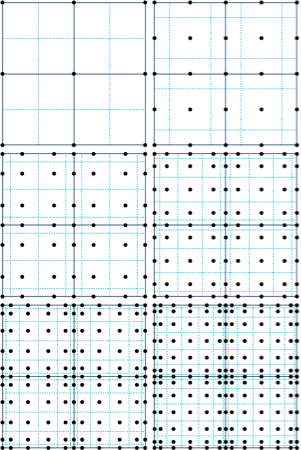
\includegraphics[clip,width=0.3\textwidth]{images/cvfem_nodes.png}
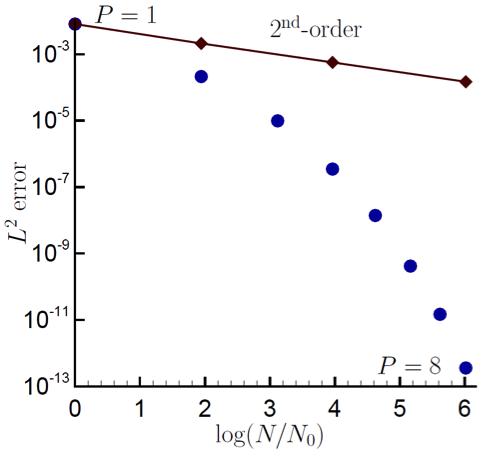
\includegraphics[clip,width=0.4\textwidth]{images/cvfem_conv.png}
\caption{Polynomial promotion for a canonical CVFEM quad element patch from $P=1$ to $P=6$ (left) and a recent spectral convergence plot using the 
Method of Manufactured Solutions for $P=1$ through $P=8$ (right).}
\label{hoCVFEM}
\end{figure}

When using CVFEM, the discretized equations described in this manual
are evaluated at either subcontrol-surface integration points (terms that
have been integrated by parts) or at the subcontrol volume (time and
source terms). Interpolation within the element is obtained by the
standard elemental basis functions,

\begin{equation}
\phi_{ip} = \sum N^{ip}_k \phi_k.
\label{cvfemInterpolation}
\end{equation}
%
where the index $k$ represents a loop over all nodes in the element.

Gradients at the subcontrol volume surfaces are obtained by taking the derivative
of Eq.~\ref{cvfemInterpolation}, to obtain,

\begin{equation}
\frac{\partial \phi_{ip}}{\partial x_j} = \sum \frac{\partial N^{ip}_{j,k}} {\partial x_j} \phi_k.
\label{cvfemDerivative}
\end{equation}

The usage of the CVFEM methods results in the canonical 27-point stencil
for a structured hexahedral mesh.

\subsection{Edge-Based Discretization}
In the edge-based discretization, the dual mesh defined in the CVFEM
method is used to pre-process both dual mesh nodal volumes (needed in
source and time terms) and edge-based area vectors (required for integrated-by-parts
quantities, e.g., advection and diffusion terms).

Consider Figure~\ref{hoCVFEM}, which is the original set of CVFEM
dual mesh quadrature points shown above. Specifically, there are four subcontrol
volumes about node 5 that contribute to the nodal volume dual mesh.
In an edge-based scheme, the time and source terms use single point
quadrature by assembling these four subcontrol volume contributions
(eight in 3D) into one single nodal volume. In most cases, source terms
may include gradients that are obtained by using the larger element-based
stencil.

The same reduction of gauss points is realized for the area vector.
Consider the edge between nodes 5 and 6. In the full CVFEM approach,
subcontrol surfaces within the top element (5,6,9,8) and bottom
element (2,3,6,5) are reduced to a single area vector at the 
edge midpoint of nodes 5 and 6. Therefore, advection and diffusion
is now done in a manner very consistent with a cell centered scheme, i.e.,
classic ``left''/''right'' states.

The consolidation of time and source terms to nodal locations along with
advection and diffusion at the edge mid-point results in a canonical
five-point stencil in 2D and seven in 3D. Note the ability to handle
hybrid meshes is readily peformed one nodal volume and edge area are
pre-processed. Edges and nodes are the sole topology that are iterated,
thus making this scheme highly efficient, although inherantly limited to 
second order spatial order of accuracy.

In general, the edge-based scheme is second order spatially accurate.
Formal verification has been done to evaluate the accuracy of the EBVC
relative to other implemented methods (Domino,~\cite{Domino:2014}). The edge-based scheme,
which is based on dual mesh post-processing, represents a commonly used finite volume 
method in gas dynamics applications. The method also lends itself to psuedo-higher order 
methodologies by the blending of extrapolated values using the projected nodal 
gradient and gauss point values (as does CVFEM). This provides a fourth order
accurate diffusion and advection operator on a structured mesh.

The use of a consistent mass matrix is less apparent in edge-based
schemes. However, if desired, the full element-based stencil can
be used by iterating elements and assembling to the nodes. 

The advantage of edge-based schemes over cell centered schemes is
that the scheme naturally allows for a mixed elemental discretization. Projected nodal gradients
can be element- or edge-based.  LES
filters and nodal gradients can also exploit the inherant elemental
basis that exists in the pure CVFEM approach. In our experience, the optimal scheme on high quality
meshes uses the CVFEM for the continuity solve and EBVC discretization for all other equations.
This combination allows for the full CVFEM diffusion operator for the pressure Poisson equation
and the EBVC approach for equations where inverse Reynolds scaling reduces the importance of the 
diffusion operator. This scheme can be activated by the use of the ``$use \textunderscore edges: yes$''
Realm line command in combination of the LowMachEOM system line command, 
``$element \textunderscore continuity \textunderscore eqs : yes$''.

\subsection{Projected Nodal Gradients}
In the edge or element-based algorithm, projected nodal gradients
are commonplace. Projected nodal gradients are used in the fourth 
order pressure stabilization terms, higher order upwind methods, discontinuity
capturing operators (DCO) and turbulence source terms. For an edge-based scheme, 
they are also used in the diffusion term when non-orthogonality of the mesh is noted.

There are many procedures for determining the projected 
nodal gradient ranging from element-based schemes to
edge-based approached. In general, the projected nodal gradient is viewed as an $L_2$ 
minimization between the discontinuous Gauss-point value and the continuous
nodal value. The projected nodal gradient, in an $L_2$ sence is given by,

\begin{equation}
\int w G_j \phi {dV} = \int \frac{\partial \phi}{\partial x_j}{dV}.
\label{PNG}
\end{equation}

Upong integration-by-parts and a piece-wise constant test function, the above equation
is written as,

\begin{equation}
\int w_I G_j \phi {dV} = \int \phi_{ip} n_j {dS}.
\label{PNG}
\end{equation}

For a lumped L2 projected nodal gradient,
the approach is based on a Green-Gauss integration,

\begin{equation}
G_j \phi = \frac{\int \phi_{ip} A_j}{dV}.
\label{greenGauss}
\end{equation}In the above lumped mass matrix approach, the value at the 
integration point can either be based on the CVFEM dual mesh 
evaluated at the subcontrol surface, i.e., the line command option, 
``$element$'' or the ``$edge$'', which evaluates the term at the edge 
midpoint using the assemble edge area vector. In all cases, the lumped mass
matrix approach is strickly second order accurate. When running higher order 
CVFEM, a consistent mass matrix appraoch is required to maintain design order 
of the overall discretization. This is strickly due to the pressure stabilization
whose accuracy can be affected by the form of the projected nodal gradient (see the Nalu
theory manual or a variety of SNL-based publications).

In the description that follows, $\bar{G_j \phi}$ represent the average nodal 
gradient evaluated at the integration point of interest.

The choice of projected nodal gradients is specified in the input file for each dof.
Keywords ``$element$'' or ``$edge$`` are used to define the form of the projection. The
forms of the projected nodal gradients is arbitrary relative to the choosed underlying
discretization. For strongly non-orthoginal meshes, it is recommended to use an element-based
projected nodal gradient for the continuity equation when the EBVC method is in use. In some limited
cases, e.g., pressure, mixture fraction and enthalpy, the $manage-png$ line command can be used to
solve the simple linear system for the consistent mass matrix.

\subsection{Time and Source Terms}
Time and source terms also volumetric contributions and also use the dual nodal volume. In both
discretization approaches, this assembly is achieved
as a simple nodal loop. In some cases, e.g., the Ksgs partial differential equation, the
source term can use projected nodal gradients.
\begin{equation}
  \int \frac{\partial \rho \phi }{\partial t} dV = \int S_{\phi}dV 
\end{equation}

\subsection{Diffusion}
As already noted, for the CVFEM method, the diffusion term at the 
subcontrol surface integration points use the the elemental
shape functions and derivatives. For the standard diffusion term, 
and using  Eq.~\ref{cvfemDerivative}, the CVFEM diffusion operator
contribution at a given integration point (here simply demonstrated 
for a 2D edge with prescribed area vector) is as follows,

\begin{eqnarray}
  -\int \Gamma \frac{\partial \phi}{\partial x_j} A_j = - \Gamma_{ip} \left[ \left(\frac{\partial N^{ip}_0} {\partial x} \phi_0 + \frac{\partial N^{ip}_1} {\partial x} \phi_1 \right) A_x + \left(\frac{\partial N^{ip}_0} {\partial y} \phi_0 + \frac{\partial N^{ip}_1} {\partial y} \phi_1 \right) A_y \right]
\end{eqnarray}

Standard Gauss point locations at the subcontrol surfaces can be shifted to the edge-midpoints for a more stable (monotonic)
diffusion operator that is better conditioned for high aspect ratio meshes. 

For the edge-based diffusion operator, special care is noted
as there is no ability to use the elemental basis to define
the diffusion operator. As with cell-centered schemes, non-orthogonal 
contributions for the diffusion operator arise due to a difference in
direction between the assembled edge area vector and the
distance vector between nodes on an edge. On skewed meshes,
this non-orthogonality can not be ignored.

Following the work of Jasek,~\cite{Jasek:1996},
the over-relaxed approach is used. The form of any gradient
for direction $j$ for field $\phi$ is

\begin{equation}
  \frac{\partial \phi}{\partial x_j}_{ip} = \bar{G_j\phi} + \left[ \left(\phi_R - \phi_L \right) 
- \bar{G_l\phi}dx_l \right] \frac{A_j}{A_k dx_k}.
\end{equation}
\label{generalGrad}

In the above expression, we are iterating edges with a Left node $L$ and Right node $R$ along
with edge-area vector, $A_j$. The $\bar{G_j \phi}$ is simple averaging of the left and right nodes
to the edge midpoint. 
In general, a standard edge-based diffusion term is written as,
\begin{eqnarray}
  -\int \Gamma \frac{\partial \phi}{\partial x_j} A_j &=& - \Gamma_{ip} \left[ \left(\bar{G_x \phi}A_x + \bar{G_y \phi}A_y \right)
    + \left( \phi_R -  \phi_L \right) \frac{A_x A_x + A_y A_y}{A_x dx_x + A_y dx_y} \right. \nonumber \\ &&
  - \left. \left( \bar{G_x \phi}dx_x + \bar{G_y \phi}dx_y \right) \frac{A_x A_x + A_y A_y} {A_x dx_x + A_y dx_y} \right].
\end{eqnarray}

\subsubsection{Momentum Stress}
The viscous stress tensor, $\tau_{ij}$ is formed based on the
standard gradients defined above for either the edge or element-based 
discretization. The viscous force for component $i$ is given by,
\begin{equation}
  -\int \tau_{ij} A_j = -\int \mu_{ip}\left( \frac{\partial u_i}{\partial x_j} + \frac{\partial u_j}{\partial x_i} \right) A_j.
\end{equation}
\label{viscousStress}
%
For example, the x and y-component of viscous force is 
given by,

\begin{eqnarray}
F_x &=& - \mu_{ip} \left( \frac{\partial u_x}{ \partial x}A_x + \frac{\partial u_x}{\partial y}A_y \right ) 
- \mu_{ip} \left( \frac{\partial u_x}{ \partial x}A_x + \frac{\partial u_y}{ \partial x}A_y \right), \\
F_y &=& - \mu_{ip} \left( \frac{\partial u_y}{ \partial x}A_x + \frac{\partial u_y}{\partial y}A_y \right ) 
- \mu_{ip} \left( \frac{\partial u_x}{ \partial y}A_x + \frac{\partial u_y}{ \partial y}A_y \right).
\end{eqnarray}

Note that the first part of the viscous stress is simply the 
standard diffusion term. Note that the so-called non-solonoidal 
viscous stress contribution is frequently written in terms of projected
nodal gradients. However, for CVFEM this procedure is rarely used 
given the elemental basis definition. As such, the use of
shape function derivatives is clear.

The viscous stress contribution at an integration point for CVFEM (again using the 2D example
with variable area vector) can be written as,

\begin{eqnarray}
  F_x &=& - \Gamma_{ip} \left[ \left(\frac{\partial N^{ip}_0} {\partial x} {u_x}_0 + \frac{\partial N^{ip}_1} {\partial x} {u_x}_1 \right) A_x + \left(\frac{\partial N^{ip}_0} {\partial y} {u_x}_0 + \frac{\partial N^{ip}_1} {\partial y} {u_x}_1 \right) A_y \right. \nonumber \\ &&
  + \left. \left(\frac{\partial N^{ip}_0} {\partial x} {u_x}_0 + \frac{\partial N^{ip}_1} {\partial x} {u_x}_1 \right) A_x + \left(\frac{\partial N^{ip}_0} {\partial y} {u_y}_0 + \frac{\partial N^{ip}_1} {\partial x} {u_y}_1 \right) A_y \right], \\ 
  F_y &=& - \Gamma_{ip} \left[ \left(\frac{\partial N^{ip}_0} {\partial x} {u_y}_0 + \frac{\partial N^{ip}_1} {\partial x} {u_y}_1 \right) A_x + \left(\frac{\partial N^{ip}_0} {\partial y} {u_y}_0 + \frac{\partial N^{ip}_1} {\partial y} {u_y}_1 \right) A_y \right. \nonumber \\ &&
  + \left. \left(\frac{\partial N^{ip}_0} {\partial y} {u_x}_0 + \frac{\partial N^{ip}_1} {\partial y} {u_x}_1 \right) A_x + \left(\frac{\partial N^{ip}_0} {\partial y} {u_y}_0 + \frac{\partial N^{ip}_1} {\partial x} {u_y}_1 \right) A_y \right].
\end{eqnarray}

For the edge-based diffusion operator, the value of
$\phi$ is substituted for the component of velocity,
$u_i$ in the Eq.~\ref{generalGrad}.

\begin{equation}
  \frac{\partial u_i}{\partial x_j}_{ip} = \bar{G_j u_i} + \left[ \left({u_i}_R - {u_i}_L \right) 
- \bar{G_l u_i}dx_l \right] \frac{A_j}{A_k dx_k}.
\end{equation}
\label{vectorGrad}
Common approaches in the cell-centered community are to use the projected nodal gradients
for the $ \frac{\partial u_j}{\partial x_i}$ stress component. However, in nalu, the above
form of equation is used.

Substituting the relations of the velocity gradients for the x and y-componnet of force above provides the
following expression used for the viscous stress contribution:

\begin{eqnarray}
  F_x &=& - \mu_{ip} \left[ \left(\bar{G_x u_x}A_x + \bar{G_y u_x}A_y \right)
    + \left( {u_x}_R -  {u_x}_L \right) \frac{A_x A_x + A_y A_y}{A_x dx + A_y dy} \right. \nonumber \\ &&
  - \left. \left( \bar{G_x u_x}dx + \bar{G_y u_x}dy \right) \frac{A_x A_x + A_y A_y} {A_x dx + A_y dy} \right] \nonumber  \\ &&
  - \mu_{ip} \left[ \bar{G_x u_x}A_x + \bar{G_x u_y}A_y + \left({u_x}_R - {u_x}_L\right) \frac{A_x A_x} {A_x dx + A_y dy} \right. \nonumber \\&&
    + \left. \left({u_y}_R - {u_y}_L\right) \frac{A_x A_y} {A_x dx + A_y dy} \right. \nonumber \\ &&
    - \left. \left( \bar{G_x u_x}dx +  \bar{G_y u_x}dy \right) \frac{A_x A_x} {A_x dx + A_y dy} \right. \nonumber \\ &&
    - \left. \left( \bar{G_x u_y}dx +  \bar{G_y u_y}dy \right) \frac{A_x A_y} {A_x dx + A_y dy} \right],
\end{eqnarray}

\begin{eqnarray}
  F_y &=& - \mu_{ip} \left[ \left(\bar{G_x u_y}A_x + \bar{G_y u_y}A_y \right)
    + \left( {u_y}_R -  {u_y}_L \right) \frac{A_x A_x + A_y A_y}{A_x dx + A_y dy} \right. \nonumber \\ &&
  - \left. \left( \bar{G_x u_y}dx + \bar{G_y u_y}dy \right) \frac{A_x A_x + A_y A_y} {A_x dx + A_y dy} \right] \nonumber \\ &&
  - \mu_{ip} \left[ \bar{G_y u_x}A_x + \bar{G_y u_y}A_y + \left({u_y}_R - {u_y}_L\right) \frac{A_y A_y} {A_x dx + A_y dy} \right. \nonumber \\&&
    + \left. \left({u_x}_R - {u_x}_L\right) \frac{A_y A_x} {A_x dx + A_y dy} \right. \nonumber \\ &&
    - \left. \left( \bar{G_x u_y]}dx +  \bar{G_y u_y}dy \right) \frac{A_y A_y} {A_x dx + A_y dy} \right. \nonumber \\ &&
    - \left. \left( \bar{G_x u_x}dx +  \bar{G_y u_x}dy \right) \frac{A_y A_x} {A_x dx + A_y dy} \right],
\end{eqnarray}
where above, the first $[]$ and second $[]$ represent the $\frac{\partial u_i}{\partial x_j}A_j$ and  
$\frac{\partial u_j}{\partial x_i}A_j$ contributions, respectively.

One can use this expression to recognize the ideal LHS sensitivities for row and columns for 
component $u_i$. 


\section{Advection Stabilization}
In general, advection for both the edge and element-based
scheme is identical with standard exception of the location of the integration
points. The full advection term is simply written as,

\begin{equation}
  ADV_{\phi} = \int \rho u_j \phi_{ip} A_j = \sum \dot{m} \phi_{ip},
\label{advForm}
\end{equation}
%
where $\phi$ is $u_i$, $Z$, $h$, etc.

The evaluation of $\phi_{ip}$ defines the advection stabilization choice. 
In general, the advection choice is a cell Peclet blending between higher
order upwind ($\phi_{upw}$) and a generalized un-stabilized central 
(Galerkin) operator, $\phi_{gcds}$,

\begin{equation}
  \phi_{ip} = \eta \phi_{upw} + (1-\eta)\phi_{gcds}.
\end{equation}
\label{advPhiIP}
%

In the above equation, $\eta$ is a cell Peclet blending. The generalized
central operator can take on a pure second order or pseudo fourth order form (see below). 
For the classic Peclet number functional form (see Equation~\ref{classicPF}) 
a hybrid upwind factor, $\gamma$, can be used to 
ensure that no stabilization is added ($\eta = 0$) or that full upwind stabilization is included (as will be shown, 
even with limiter functions). The hybrid upwind factor allows one to modify the functional
blending function; values of unity result in the normal blending function 
response in  Figure~\ref{pec-blend}; values of zero yield
a pure central operator, i.e., blending function of zero; values $>>$ unity result 
in a blending function value of unity, i.e., pure upwind. The constant $A$
is implemented with a value of 5. The value of this constant can not be changed
via the input file. Note that this functional form is named the ``classic'' form
within the input file.

The classic cell Peclet blending function is given by
\begin{equation}
  \eta = \frac {{\gamma \rm Pe}^2} {5 + {\gamma \rm Pe}^2}.
\label{classicPF}
\end{equation}
The classic Peclet functional form makes it difficult to dial in the exact
point at which the Peclet factor transitions from pure upwind to pure central. 
Therefore, an alternative form is provided that has a hyperbolic tangeant 
functional form. This form allows one to specify the transition point and 
the width of the transition (see Equation~\ref{tanhPF}).
The tanh form is as follows,
\begin{equation}
  \eta = \frac {\frac {1}{2}[1+tanh(\frac{\rm Pe - c_{trans}}{c_{width}})] -\lambda}{\delta}.
\label{tanhPF}
\end{equation}
Above, the constant $c_{trans}$ represents the transition Peclet number while $c_{width}$ represents the width of 
the transition. The value of $\lambda$ is simply the shift between of the raw tanh function
from zero while $\delta$ is the difference between the max Peclet factor (unity) and the minimum value
prior to normalization. This approach ensures that the function starts at zero and asymptotes to unity. 

The cell-Peclet number is computed for each sub-face in the element
from the two adjacent left (L) and right (R) nodes,
\begin{equation}
   {\rm Pe} = {{{1 \over 2} \left( u_{R,i} + u_{L,i} \right) 
                      \left( x_{R,i} - x_{L,i} \right) } \over \nu }.
\end{equation}
A dot-product is implied by repeated indices. 

\begin{figure} [h]
\centerline{\includegraphics[height=3.0in]{images/pecletFactor}}
\vspace{0.1in}
\caption{Cell-Peclet number blending function outlining classic (varying the hybrid factor $\gamma$ from 1.0, 0.1 and 0.01; again $A=5$) and tanh functional form ($c_{trans}=2000$ and $c_{width}=200$).}
\label{pec-blend}
\end{figure}
 
The upwind operator, $\phi_{upw}$ is computed based on a blending of the extrapolated
state (using the projected nodal gradient) and the linear interpolated state. Second 
or third order upwind is provided based on the value of $\alpha_{upw}$ blending
\begin{eqnarray}
 \phi_{upw} = \alpha_{upw}\tilde \phi^L_{upw} + \left(1-\alpha_{upw}\right)\phi_{cds}; \dot m > 0, \nonumber \\
             \alpha_{upw}\tilde\phi^R_{upw} + \left(1-\alpha_{upw}\right)\phi_{cds}; \dot m < 0.
\label{phiUpwindFull}
\end{eqnarray}
The extrapolated value based on the upwinded left ($\phi^L$) or right ($\phi^R$) state,

\begin{eqnarray}
  \tilde \phi^L_{upw} = \phi^L + d^L_j \frac{\partial \phi^L }{\partial x_j}, \nonumber \\
  \tilde \phi^R_{upw} = \phi^R - d^R_j \frac{\partial \phi^R }{\partial x_j}.
\label{advUpwLR}
\end{eqnarray}
%
The distance vectors are defined based on the distances between the L/R points and the integration point 
(for both edge or element-based),
\begin{eqnarray}
  d^L_j = x^{ip}_j - x^L_j, \nonumber \\
  d^R_j = x^R_j - x^{ip}_j. 
\end{eqnarray}
\label{distanceVec}
In the case of all transported quantities, a Van Leer limiter of the extrapolated value is supported
and can be activated withing the input file (using the solution options ``limiter'' specification).

Second order central is simply written as a linear combination of the nodal values,
\begin{equation}
 \phi_{cds} = \sum N^{ip}_k \phi_k.
\label{phiCentral}
\end{equation}
%
where $N^{ip}_k$ is either evaluated at the subcontrol surface or edge midpoint. In the case
of the edge-based scheme, the edge midpoint evaluation provides for a skew symmetric form
of the operator. 

The generalized central difference operator is provided by blending with the extrapolated values and 
second order Galerkin,
\begin{equation}
 \phi_{gcds} = \frac{1}{2} \left(  \hat\phi^L_{upw} + \hat\phi^R_{upw} \right),
\label{phi4th}
\end{equation}
where,
\begin{eqnarray}
  \hat\phi^L_{upw} = \alpha \tilde \phi^L_{upw} + \left(1-\alpha\right) \phi_{cds}, \nonumber \\
  \hat\phi^R_{upw} = \alpha \tilde \phi^R_{upw} + \left(1-\alpha\right) \phi_{cds}.
\label{advNew4th}
\end{eqnarray}
The value of $\alpha$ provides the type of psuedo fourth order stencil and is specified in the user
input file.

The above set of advection operators can be used to define an idealized one dimensional stencil denoted
by ($i-2$, $i-1$, $i$, $i+1$, $i+2$), where $i$ represents the particular row for the given transported
variable. Below, in Table~\ref{tab-stencil} the stencil can be noted for each value of $\alpha$ and $\alpha_{upw}$.


\begin{table}[h]
 \caption{Edge-based stencils for various combinations of $\alpha$ and $\alpha_{upw}$}
 \label{tab-stencil}
 \vspace{0.1in}
 \centerline{
  \begin{tabular}{|l|l|l|l|l|l|l|} \hline
    $i-2$             &  $i-1$           &  $i$            & $i+1$           &  $i+2$           & $\alpha$      & $\alpha_{upw}$ \\ \hline
    $0$               &  $-\frac{1}{2}$  &  $0$            & $+\frac{1}{2}$  &  $0$             & $0$           & $n/a$          \\ \hline
    $+\frac{1}{8}$    &  $-\frac{6}{8}$  &  $0$            & $+\frac{6}{8}$  &  $-\frac{1}{8}$  & $\frac{1}{2}$ & $n/a$          \\ \hline
    $+\frac{1}{12}$   &  $-\frac{8}{12}$ &  $0$            & $+\frac{8}{12}$ &  $-\frac{1}{12}$ & $\frac{2}{3}$ & $n/a$          \\ \hline
    $+\frac{1}{4}$    &  $-\frac{5}{4}$  &  $+\frac{3}{4}$ & $+\frac{1}{4}$  &  $0$             & $\dot m > 0$  & $1$ \\ \hline
    $0$               &  $-\frac{1}{4}$  &  $-\frac{3}{4}$ & $+\frac{5}{4}$  &  $-\frac{1}{4}$  & $\dot m < 0$  & $1$ \\ \hline
    $+\frac{1}{6}$    &  $-\frac{6}{6}$  &  $+\frac{3}{6}$ & $+\frac{2}{6}$  &  $0$             & $\dot m > 0$  & $\frac{1}{2}$ \\ \hline
    $0$               &  $-\frac{2}{6}$  &  $-\frac{3}{6}$ & $+\frac{6}{6}$  &  $-\frac{1}{6}$  & $\dot m < 0$  & $\frac{1}{2}$ \\ \hline
  \end{tabular}
 }
\end{table}

It is noted that by varying these numerical parameters, both high quality, low dissipation operators
suitable for LES usage or limited, monotonic operators suitable for RANS modeling can be accomodated.


\section{Pressure Stabilization}
A number of papers describing the pressure stabilization approach that Nalu uses are in the open literature,
Domino,~\cite{Domino:2006, Domino:2008, Domino:2014}.  Nalu supports an incremental
fourth order approximate projection scheme with time step 
scaling. By scaling, it is implied that a time scale based on either the physical time step or 
a combined elemental advection and diffusion time scale based on element length along
with advection and diffusional parameters. An alternative to the approaximate projection
concept is to view the method as a variational multiscale (VMS) method wherebye the momentum residual
augments the continuity equation. This allows for a diagonal entry for the pressure degree of freedom.

Here, the fine-scale momentum residual is written in terms of a projected momentum residual 
evaluated at the Gauss point,
\begin{equation}
  \mathbf{R}(u_i) = (\frac{\partial p} {\partial x_j} - G_j p ).
\label{fineScaleMomentum}
\end{equation}
The above equation is derived simply by writing a fine-scale momentum equation at the Gauss-points 
and using the nodal projected residual to reconstruct the individual terms.
Therefore, the continuity equation solved, using the VMS-based projected momentum residual, is

\begin{equation}
\int \frac{\partial \bar{\rho}} {\partial t}\, dV
+ \int \left( \bar{\rho} \hat{u}_i + \tau G_i \bar{P} \right) n_i\, dS
  = \int \tau \frac{\partial \bar{P}}{\partial x_i} n_i\, dS.
\end{equation}
%
Above, $G_i \bar{P}$ is defined as a L2 nodal projection of the pressure gradient. Note that the notion of 
a provisional velocity, $\hat u_i$, is used to signify that this velocity is the product of the momentum 
solve. The difference between the projected nodal gradient interpolated to the gauss point and the 
local gauss point pressure gradient provides a fourth order pressure stabilization
term. This term can also be viewed as an algebraic form for the momentum residual. For the continuity
equation only, a series of element-based options that shift the integration points to the edges of the 
iterated element is an option.

\subsection{The Role of $\dot m$}

In all of the above equations, the advection term is written in terms of a linearized 
mass flow rate including a sum over all subcontrol surface integration points,
Eq.~\ref{advForm}. The mass flow rate includes the full set of stabilization terms
obtained from the continuity solve,
\begin{equation}
\dot m = \left(\bar{\rho} \hat{u}_i + \tau G_i \bar{P} 
  -\tau \frac{\partial \bar{P}}{\partial x_i}\right) n_i\, dS.
\end{equation}
The inclusion of the pressure stabilization terms in the advective
transport for the primitives is a required step for ensuring that
the advection velocity is mass conserving. In practive, the mass flow
rate is stored at each integration point in the mesh (edge midpoints for the
edge-based scheme and subcontrol surfaces for the element-based scheme).
When the mixed CVFEM/EBVC scheme is used, the continuity equation solves for
a subcontrol-surface value of the mass flow rate. These values are assembled to the
edge for use in the EBVC discretization approach. Therefore, the storage for mass
flow rate is higher.



\section{RTE Stabilization}
The RTE is solved using the method of discrete ordinates using the symmetric
Thurgood quadrature set. The discrete ordinates method is one in which
discrete directions of the intensity are solved. The quadrature order, $N$,
defines the number of ordinate directions that are solved in a given 
iteration. In the case of non-scattering media, this results is a set
of decoupled linear partial differentail equations. For the symmetric
Thurgood set, the number of ordinate directions is given by $8N^2$. Values
of N that are required for suitable accuracy starts at $N=2$ with more than
adequate resolution at $N=4$.

For each ordinate direction, a weight is provided, $w_k$ (not to be confused with the
test function $w$). For each intensity ordinate direction,
$I_k$, integrated quantities such as scalar flux and radiative heat flux are computed as,

\begin{equation}
G = \sum I_k w_k
\end{equation}
and,
\begin{equation}
  q_j = \sum I_k s_j w_k.
\end{equation}

The stabilization that is used in the RTE equation can be placed in the
class of residual-based stabilization. In this particular implementation,
the scaled residual of the RTE equation is added. This implementation
has its roots in the classic variational multiscale (VMS). 

In the VMS framework, the degree of freedom is decomposed in terms of its 
resolved and fine scale, $I+I'$. Without specific definition of the test function, 
the weighted residual statement for the RTE within a VMS framework is given by,
\begin{equation}
   \int w \left( s_i {{\partial} \over {\partial x_i}} \left(I\left(s\right) + I'\left(s\right)\right)
   + (\mu_a + \mu_s) \left(I\left(s\right) + I'\left(s\right)\right) - {{\mu_a \sigma T^4} \over {\pi}} -\frac{\mu_s}{4\pi}G \right) {\rm d}V = 0.
\label{rteVMS}
\end{equation}
%
Grouping resolved and fine scale terms results in an equation takes the form of a standard Galerkin 
contribution in addition to the fine structure statement,
\begin{eqnarray}
   \int w \left( s_i {{\partial} \over {\partial x_i}} I\left(s\right)
   + (\mu_a + \mu_s)I - {{\mu_a \sigma T^4} \over {\pi}} -\frac{\mu_s}{4\pi}G \right) {\rm d}V  \nonumber \\ 
   + \int w \left( s_i {{\partial} \over {\partial x_i}} I'\left(s\right)
   + (\mu_a + \mu_s) I' \right) {\rm d}V  = 0.
\label{rteVMS1}
\end{eqnarray}
%
Note that the isotropic source term has not contributed to the VMS framework other than through
the right hand source term.

In general, gradients in the fine scale quantity are to be avoided. Therefore, the first term
in the second line of Eq.~\ref{rteVMS1} is integrated by parts to yield the following
form (note the boundary term, $\int_\Gamma$ that is shown below is frequently dropped)
\begin{eqnarray}
   \int w \left( s_i {{\partial} \over {\partial x_i}} I\left(s\right)
   + (\mu_a +\mu_s)I - {{\mu_a \sigma T^4} \over {\pi}} -\frac{\mu_s}{4\pi}G \right) {\rm d}V  \nonumber \\ 
   - \int I' s_i {{\partial w} \over {\partial x_i}} {\rm d}V 
   + \int_{\Gamma} w s_i I' n_i {\rm d}S + \int w (\mu_a + \mu_s)I' {\rm d}V  = 0.
\label{rteVMS2}
\end{eqnarray}
The following ansatz, which now includes the classic stabilization parameter, $\tau$,
provides closure of the above fine scale equation,
\begin{equation}
   I' = -\tau\left(s_i {{\partial} \over {\partial x_i}} I\left(s\right) + (\mu_a + \mu_s)I\left(s\right) 
   - {{\mu_a \sigma T^4} \over {\pi}} -\frac{\mu_s}{4\pi}G \right) = -\tau R(s)
\label{fineScaleClosure}
\end{equation}
%
 Substituting Eq.~\ref{fineScaleClosure} into Eq.~\ref{rteVMS2} yields,
\begin{eqnarray}
   \int w \left( s_i {{\partial} \over {\partial x_i}} I\left(s\right)
   + (\mu_a +\mu_s)I - {{\mu_a \sigma T^4} \over {\pi}} -\frac{\mu_s}{4\pi}G \right) {\rm d}V  \nonumber \\ 
   + \int \tau s_i {{\partial w} \over {\partial x_i}} R(s) {\rm d}V 
   - \int_\Gamma \tau w R(s) s_i n_i {\rm d}S - \int \tau w (\mu_a + \mu_s)R(s) {\rm d}V  = 0.
\label{rteVMS3}
\end{eqnarray}
In the above equation, the residual of the intensity equation for ordinate $s$
is denoted by $R(s)$. A compact form of the equation is provided by defining a modified
test function, $\tilde w$, (again note retention of the stabilized boundary term)
\begin{eqnarray}
   \int \tilde w \left( s_i {{\partial} \over {\partial x_i}} I\left(s\right)
   + (\mu_a + \mu_s)I - {{\mu_a \sigma T^4} \over {\pi}} -\frac{\mu_s}{4\pi}G \right) {\rm d}V \nonumber \\
 - \beta \int_\Gamma \tau w R(s) s_i n_i {\rm d}S = 0.
\label{rteVMSCompact}
\end{eqnarray}
where $\tilde w$ is simply equal to,
\begin{equation}
   \tilde w  = w + \tau \left( s_j \frac{\partial w }{\partial x_j} + \alpha (\mu_a + \mu_s)w \right).
\label{modW}
\end{equation}
When $\alpha = -1$, we have the above VMS derivation; for $\alpha = 1$, Galerkin Least Squares is realized;
finally for $\alpha = 0$, we have SUPG. For any formulation other than VMS, the residual contribution
at the boundaries of the domain is dropped ($\beta = 0$).

The full residual-based equation is placed in divergence form,
\begin{eqnarray}
   \int \tilde w \left( {{\partial} \over {\partial x_i}} s_i I\left(s\right)
   + (\mu_a + \mu_s) I\left(s\right) - {{\mu_a \sigma T^4} \over {\pi}} -\frac{\mu_s}{4\pi}G \right) {\rm d}V \nonumber \\
   - \beta \int_\Gamma \tau w R(s) s_i n_i {\rm d}S = 0.
\label{rteDivForm}
\end{eqnarray}
and split into its Galerkin and stabilized contributions,
\begin{eqnarray}
   \int w \left( {{\partial} \over {\partial x_i}} s_i I\left(s\right)
   + (\mu_a + \mu_s )I\left(s\right) - {{\mu_a \sigma T^4} \over {\pi}} -\frac{\mu_s}{4\pi}G \right) {\rm d}V \nonumber \\
 +\int \tau s_j \frac{\partial w }{\partial x_j} R(s) {\rm d}V \nonumber \\
+\alpha\int \tau w (\mu_a + \mu_s)R(s) {\rm d}V \nonumber \\
- \beta \int_\Gamma \tau w R(s) s_i n_i {\rm d}S = 0.
\label{rteDivFormSub}
\end{eqnarray}
Note that the first term in the above equation is integrated by parts,
\begin{equation}
\int w {{\partial} \over {\partial x_i}} s_i I\left(s\right) {\rm d}V = -\int I\left(s\right) s_i \frac{\partial w}{\partial x_i} {\rm d}V 
+ \int_{\Gamma} w s_i I\left(s\right) n_i {\rm d}S.
\end{equation}
Again, the usage of $\Gamma$ provides emphasis that the contribution is a boundary (exposed face) condition. 
Therefore, the full VMS-based stabilized RTE equation is as follows,
\begin{eqnarray}
   \int \left( -I\left(s\right) s_i \frac{\partial w}{\partial x_i} + w [(\mu_a + \mu_s) I\left(s\right) 
- {{\mu_a \sigma T^4} \over {\pi}} -\frac{\mu_s}{4\pi}G ] \right) {\rm d}V  \nonumber \\
+ \int_\Gamma w s_i I\left(s\right) n_i {\rm d}S \nonumber \\
 +\int \tau s_j \frac{\partial w }{\partial x_j} R(s) {\rm d}V \nonumber \\
+\alpha\int \tau w (\mu_a + \mu_s)R(s) {\rm d}V \nonumber \\
- \beta \int_\Gamma \tau w R(s) s_i n_i {\rm d}S = 0.
\label{rteDivFormSub}
\end{eqnarray}

\subsubsection{Definition of the CVFEM test function}
Following the work of Martinez,~\cite{Martinez:2005}, the test function is chosen to be a 
piecewise-constant value within the control volume, $w = w_I$ and zero outside of this control volume (Heaviside).
A key property of this function, as pointed out by Martinez, is that its
gradient is a distribution of delta functions on the control volume
boundary:
\begin{equation}
\frac{\partial w_I}{\partial x_i} = - {\bf n}_I \delta({\bf x} - {\bf x}_{\Gamma_I})
\label{eqn:GradPiecewiseConstant}
\end{equation}
where $\Gamma_I$ is boundary of control volume $I$ and ${\bf n}_I$
is the outward normal on that boundary.  Substituting this relationship into the residual equation provides
the final form of vertex-centered finite volume RTE stabilized equation,

\begin{eqnarray}
   \int I\left(s\right) s_i n_i {\rm d}S + \int \left( (\mu_a + \mu_s ) I\left(s\right) 
   - {{\mu_a \sigma T^4} \over {\pi}} -\frac{\mu_s}{4\pi}G \right) {\rm d}V  \nonumber \\
+ \int_\Gamma s_i I\left(s\right) n_i {\rm d}S \nonumber \\
 - \int \tau R(s) s_i n_i {\rm d}S +\alpha \int \tau (\mu_a +\mu_s) R(s) {\rm d}V -\beta \int_\Gamma \tau R(s) s_i n_i {\rm d}S= 0.
\label{rteSUCVForm}
\end{eqnarray}
Given this equation, either an edge-based or element-based scheme can be used. For $\alpha = 0$ and $\beta = 0$, it 
is noted that classic SUCV is obtained. The second line of Eq.~\ref{rteSUCVForm} represents a boundary contribution. 
This is where the intensity boundary condition (Eq.~\ref{intBc}) is applied. As noted in the RTE equation section, 
when $s_j n_j$ is greater than zero, the interpolated intensity based on
the surface nodal values is used. However, when $s_j n_j$ is less than zero, the intensity boundary condition 
value is used. Since the original RTE equation was integrated 
by parts, a natural surface flux contribution is applied. In alternative discretization approaches, e.g., the
SUPG FEM-based Sierra Thermal Radiation Module: Syrinx code, the RTE is not integrated by parts. Therefore, 
no boundary term exists, and, therefore, a dirichlet bc is applied. At corner nodes, this approach can lead 
to non-intuitive approaches since the corner node might have surface facets that are both incoming and outgoing. 
Weak integration of the flux term eliminated this complexity.

\subsubsection{The form of $\tau$}
The value of the stabilization parameter $\tau$ can take on a variety of forms. 
A classic derivation provides the form of $\tau$ to be broken out into two forms, 
$\tau_{adv} = \frac{h}{2}$ and $\tau_{diff} = \frac{1}{(\mu_a+\mu_s)}$. An ad-hoc blending 
is given by,
\begin{equation}
   \tau  = \left( \frac{1} {\frac{2}{h}^2 + (\mu_a+\mu_s)^2} \right)^ \frac{1}{2}
\label{blendedTau}
\end{equation}

Finally, the classic GFEM form of $\tau$ is given by use of the metric tensor for the element mapping is noted,

\begin{equation}
   \tau = \beta^* [s_i g_{ij}s_j]^{-\frac{1}{2}},
\label{farzin}
\end{equation}
with $\beta^*$ equal to unity for SUCV and $\frac{2}{15^{\frac{1}{2}}}$ for FEM.

\subsection{Pure Edge-based Upwind Method}
The residual-based stabilization apporach can lead to predicting negative intensities. This is simply due 
to the fact that the stabilization approach (SUPG) is a linear approach. Extensions of this residual-based
stabilization to include a discontinuity capturing operator (DCO) are underway. This adds a non-linear stabilization
approach that will, hopefully, eliminate negative intensity predictions. 

Alternatively, a first order upwind approach has been implemented by using EBVC discretization. At this point, 
no higher order upwind extensions have been implemented. For the upwind implementation, the equation solved is,

\begin{eqnarray}
   \int I\left(s\right) s_i n_i {\rm d}S + \int \left( (\mu_a + \mu_s ) I\left(s\right) 
   - {{\mu_a \sigma T^4} \over {\pi}} -\frac{\mu_s}{4\pi}G \right) {\rm d}V  \nonumber \\
+ \int_\Gamma s_i I\left(s\right) n_i {\rm d}S  = 0.
\label{rteSUCVForm}
\end{eqnarray}
In the above equation, the ``advection operator'', $I\left(s\right) s_i n_i {\rm d}S$ is
approximated as using the ``upwind'' intensity, e.g., if $s_j n_j$ is greater than zero, 
the left nodal value is used.

\subsection{Finite Element SUPG Form}
For the FEM, the test function is the standard weighting. Assuming a pure SUPG formulation, i.e.,
$\alpha = \beta = 0$ in Equation~\ref{rteDivFormSub}, thereby reducing the final form to the following:

\begin{eqnarray}
   \int \left( -I\left(s\right) s_i \frac{\partial w}{\partial x_i} + w[(\mu_a + \mu_s) I\left(s\right) 
- {{\mu_a \sigma T^4} \over {\pi}} -\frac{\mu_s}{4\pi}G ] \right) {\rm d}V  \nonumber \\
+ \int_\Gamma w s_i I\left(s\right) n_i {\rm d}S \nonumber \\
 +\int \tau s_j \frac{\partial w }{\partial x_j} R(s) {\rm d}V \nonumber \\
\label{rteFemSUPG}
\end{eqnarray}
The weak boundary condition is applied in a similar manner as with the CVFEM and EBVC form, however,
using the appropriate FEM test test function definition. Finally, the form of $\tau$ follows the above
CVFEM form.


\section{Nonlinear Stabilization Operator (NSO)}
An alternative to classic Peclet number blending is the usage of a discontinuity 
capturing operator (DCO), or in the low Mach context a nonlinear stabilization 
operator (NSO). In this method, an artifical viscosity is defined that is a function 
of the local residual and scaled computational gradients. Viable usages for the NSO 
can be advection/diffusion problems in addition to the aforementioned RTE VMS approach.

The formal finite element kernel for a NSO approach is as follows,
\begin{equation}
  \sum_e \int_\Omega \nu(\mathbf{R}) \frac{\partial w}{\partial x_i} g^{ij} \frac{\partial \phi} {\partial x_j} d\Omega,
\label{nsoFEMForm}
\end{equation}
where $\nu(\mathbf{R})$ is the artifical viscosity which is a function of the pde fine-scale 
residual and $g^{ij}$ is the covariant metric tensor).

For completeness, the covariant and contravarient metric tensor are given by,
\begin{equation}
  g^{ij} = \frac{\partial x_i} {\partial \xi_k}\frac{\partial x_j} {\partial \xi_k},
\label{coVariant}
\end{equation}

 and

\begin{equation}
  g_{ij} = \frac{\partial \xi_k} {\partial x_i} \frac{\partial \xi_k} {\partial x_j},
\label{coVariant}
\end{equation}

where $\xi = (\xi_1, \xi_2, \xi_3)^T$.
%
The form of $\nu(\mathbf{R})$ currently used is as follows,
\begin{equation}
  \nu = \sqrt{ \frac{\mathbf{R_k} \mathbf{R_k}} {\frac {\partial \phi}{\partial x_i} g^{ij} \frac{\partial \phi}{\partial x_j}} }.
\label{nuOne}
\end{equation}
The classic paper by Shakib (~\cite{Shakib:1991}) represents the genesis of this method which was done 
in the accoustically compressible context.

A residual for a classic advection/diffusion/source pde is simply the fine scale residual 
computed at the gauss point,
\begin{equation}
 \mathbf{\hat R} = \frac{\partial \rho \phi}{\partial t} + \frac{\partial}{\partial x_j} (\rho u_j \phi - \mu^{eff} \frac{\partial \phi}{\partial x_j}) -S
 \label{nsoResidual}
\end{equation}
Note that the above equation requires a second derivative whose source is the 
diffusion term. The first derivative is generally determined by using projected 
nodal gradients. As will be noted in the pressure stabilization section, the advection 
term carries the pressure stabilization terms. However, in the above equation, these 
terms are not explicity noted. Therefore, an option is to subtract the fine scale 
continuity equation to obtain the final general form of the source term,
\begin{equation}
 \mathbf{R} = \mathbf{\hat R} - \phi (\frac{\partial \rho}{\partial t} + \frac{\partial \rho u_j }{\partial x_j}).
 \label{nsoResidual}
\end{equation}

An alternative to the fine-scale PDE is a form that is found by differencing the linearized
form of the residual from the nonlinear residual,
\begin{equation}
 \mathbf{R} = \frac{\partial \rho u_j \phi }{\partial x_j} - (\phi \frac{\partial \rho u_j }{\partial x_j} + \rho u_j \frac{\partial \phi}{\partial x_j}).
 \label{nsoResidualAlt}
\end{equation}
The above resembles a commutation error in the nonlinear advection term.

In general, the NSO-$\nu$ is prone to percision issues when the gradients are very close to 
zero. As such, the value of $\nu$ is limited to a first-order like value. This parameter is 
proposed as follows: if an operator were written as a Galerkin (un-stabilized) plus a diffusion 
operator, what is the value of the diffusion coefficient such that first-order upwind is obtained 
for the combined operator? This upwind limited value of $\nu$ provides the highest value that 
this coefficient can (or should) be. The current form of the limited upwind $\nu$ is as follows,

\begin{equation}
  \nu^{upw} = C_{upw}(\rho u_i g_{ij} \rho u_j )^{\frac{1}{2}}
\label{nsoFVForm}
\end{equation}
where $C_{upw}$ is generally taked to be ~0.1.

Using a piecewise-constant test function suitable for CVFEM and EBVC schemes (the reader is refered to 
the VMS RTE section), Eq.~\ref{nsoFEMForm} can be written as,
\begin{equation}
  -\sum_e \int_\Gamma \nu(\mathbf{R}) g^{ij} \frac{\partial \phi} {\partial x_j} n_i dS.
\label{nsoFVForm}
\end{equation}
%
A fourth order form, which writes the stabilization as the difference between the Gauss-point gradient 
and the projected nodal gradient interpolated to the Gauss-point, is also supported,
\begin{equation}
  -\sum_e \int_\Gamma \nu(\mathbf{R}) g^{ij} (\frac{\partial \phi} {\partial x_j} - G_j \phi ) n_i dS.
\label{nsoFVForm4th}
\end{equation}

\subsection{NSO Based on Kinetic Energy Residual}
An alternative formulation explored is to share the general kernal form shown in Equation~\ref{nsoFVForm4th},
however, compute $\nu$ based on a fine-scale kinetic energy residual. In this formulation, the fine-scale
kinetic energy residual is obtained from the fine-scale momentum residual dotted with velocity. As with the 
continuity stabilization approach, the fine-scale momentum residual is provided by Equation~\ref{fineScaleMomentum}.
Therefore, the fine-scale kinetic energy is written as,
\begin{equation}
 \mathbf{R}_{ke} = \frac{u_j(\frac{\partial p} {\partial x_j} - G_j p )}{2 \rho},
\label{fineScaleKe}
\end{equation}
while the denominator for $\nu$ now includes the gradient in ke,
\begin{equation}
  \nu = \sqrt{ \frac{\mathbf{R}_{ke} \mathbf{R}_{ke}} {\frac {\partial ke}{\partial x_i} g^{ij} \frac{\partial ke}{\partial x_j}} }.
\label{nuKe}
\end{equation}
The kinetic energy is simply given by,
\begin{equation}
  ke = \frac{u_k u_k}{2}
\label{keForm}
\end{equation}

The kinetic energy form of $\nu$ is used for all equation sets with transformation by usage of a 
turbulent Schmidt/Prandtl number.

\subsection{Local or Projected NSO Diffusive Flux Coefficient}
While the NSO kernel is certainly evaluated at the subcontrol surfaces, the evaluation of $\nu$ can be 
computed by a multitude of approaches. For example, the artificial diffusive flux coefficient 
can be computed locally (with local residuals and local metric tensors) or can be projected 
to the nodes (via an $L_{oo}$ or $L_2$ projection) and re-interpolated to the gauss points. 
The former results in a sharper local value while the later results in a more filtered-like value.
The code base only supports a local NSO $\nu$ calculation.

\subsection{General Findings}
In general, the NSO approach seems to work best when running the fourth-order option as the second-order 
implementation still looks more diffuse. When compared to the standard MUSCL-limited scheme, the NSO
is the preferred choice. More work is underway to improve stabilization methods.
Note that a limited set of NSOs are activated in the code base with specific
interest on scalar transport, e.g, momentum, mixture fraction and static enthalpy transport. 
When using the $4^{th}$  order method, the consistent mass matrix approach for the projected 
nodal gradients is supported for higher order.

\subsection{NSO as a Turbulence Model}
The kinetic energy residual form has been suggested to be used as a turbulence model (Guermond and Larios, 2015). However,
inspection of the above NSO kernel form suggests that the model form is not symmetric. Rather, in the context of
turbulence modeling, is closer to the metric tensor acting on the difference between the rate of strain and antisymmetric
tensor. As such, the theory developed, e.g., for eigenvalue perturbations of the stress tensor (see Jofre and Domino, 2017) can not be applied. In this section,
a new form of the NSO is provided in an effort to be used for an LES closure.

In this proposed NSO formulation, the subgrid stress tensor, $\tau^{sgs}_{ij} = \overline{u_i u_j} - \bar u_i \bar u_j$, 
is given by,
\begin{equation}
  \tau^{sgs}_{ij} = - 2 \rho \nu g^{ij} (S_{ij} - \frac{1}{3}\frac{\partial u_k} {\partial x_k} \delta_{ij}) 
                = - 2 \rho \nu g^{ij} S^*_{ij}.
\label{nsoTurbForm}
\end{equation}
Interestingly, the units of $\nu$ are of an inverse time scale while the product $2 \rho \nu g^{ij}$ can be viewed
as an non-isotropic eddy viscosity, $\mu^t_{ij}$.

The first order clipping may be relaxed by defining $\nu$ as,
\begin{equation}
  \nu = \frac{| \mathbf{R}_{ke} |} {||ke||_\infty}.
\label{nuTurb}
\end{equation}
The above form would be closer to what Guermond uses and would avoid the divide-by-zero noted in regions of uniform flow.






\section{Turbulence Modeling}

Unlike a RANS approach which models most or all of the turbulent
fluctuations, LES directly solves for all resolved turbulent length 
scales and only models the smallest scales below the grid size.  In this
way, a majority of the problem-dependent, energy-containing turbulent
structure is directly solved in a model-free fashion.  The subgrid scales
are closer to being isotropic than the resolved scales, and they generally
act to dissipate turbulent kinetic energy cascaded down from the larger
scales in momentum-driven turbulent flows.  Modeling
of these small scales is generally more straightforward than RANS 
approaches, and overall solutions are usually more tolerant to LES
modeling errors because the subgrid scales comprise such a small portion
of the overall turbulent structure.  While LES is
generally accepted to be much more accurate than RANS approaches for 
complex turbulent flows, it is also significantly more expensive
than equivalent RANS simulations due to the finer grid resolution
required.  Additionally, since LES results in a full unsteady solution,
the simulation must be run for a long time to gather any desired 
time-averaged statistics.  The tradeoff between accuracy and cost 
must be weighed before choosing one method over the other.

The separation of turbulent length scales required for LES is obtained
by using a spatial filter rather than the RANS temporal filter.
This filter has the mathematical form
%
\begin{equation} 
\overline{\phi(\boldsymbol{x},t)} \equiv \int_{-\infty}^{+\infty}
    \phi(\boldsymbol{x}',t) G(\boldsymbol{x}' - \boldsymbol{x})\,
    \mathrm{d}\boldsymbol{x}',
\label{les-filter}
\end{equation}
%
which is a convolution integral over physical space $\boldsymbol{x}$
with the spatially-varying filter function $G$.  The filter function
has the normalization property $\int_{-\infty}^{+\infty}
G(\boldsymbol{x})\, \mathrm{d}\boldsymbol{x} = 1$, and it has a characteristic
length scale $\Delta$ so that it filters out turbulent length scales
smaller than this size.  In the present formulation, a simple ``box filter''
is used for the filter function,
%
\begin{equation}
G(\boldsymbol{x}' - \boldsymbol{x}) = \left\{ \begin{array}{l@{\quad:\quad}l}
    1/V         & (\boldsymbol{x}' - \boldsymbol{x}) \in \mathcal{V} \\
    0           & \mathrm{otherwise} \\
    \end{array} \right.,
\end{equation}
%
where $V$ is the volume of control volume $\mathcal{V}$ whose central 
node is located at $\boldsymbol{x}$.  This is essentially an unweighted
average over the control volume.  The length scale of this filter
is approximated by $\Delta = V^\frac{1}{3}$.  This is typically called 
the grid filter, as it filters out scales smaller than the 
computational grid size.

Similar to the RANS temporal filter, a variable can be represented in 
terms of its filtered and subgrid fluctuating components as
%
\begin{equation}
\phi = \bar{\phi} + \phi'.
\end{equation}
%
For most forms of the filter function $G(\boldsymbol{x})$,
repeated applications of the grid filter to a variable do not yield the
same result.  In other words, $\bar{\bar{\phi}} \ne 
\bar{\phi}$ and therefore $\overline{\phi'} \ne 0$, unlike with the 
RANS temporal averages.

As with the RANS formulation, modeling is much simplified in the
presence of large density variations if a Favre-filtered approach is used.
A Favre-filtered variable $\tilde{\phi}$ is defined as
%
\begin{equation}
\tilde{\phi} \equiv \frac{ \overline{\rho\phi} }{ \bar{\rho} }
\end{equation}
%
and a variable can be decomposed in terms of its Favre-filtered and
subgrid fluctuating component as
%
\begin{equation}
\phi = \tilde{\phi} + \phi''.
\end{equation}
%
Again, note that the useful identities for the Favre-filtered RANS
variables do not apply, so that $\bar{\tilde{\phi}} \ne \tilde{\phi}$
and $\overline{\phi''} \ne 0$.  The Favre-filtered approach is used for
all LES models in Nalu.

\subsection{Standard Smagorinsky LES Model}

The standard Smagorinsky LES closure model approximates the subgrid
turbulent eddy viscosity using a mixing length-type model, where the 
LES grid filter size $\Delta$ provides a natural length scale.  The
subgrid eddy viscosity is modeled simply as (Smagorinsky)
%
\begin{equation}
\mu_t = \rho \left(C_s \Delta \right)^2 | \tilde {S} |,
\label{mut-smag}
\end{equation}
%
The constant coefficient $C_s$ typically varies between $0.1$ and
$0.24$ and should be carefully tuned to match the problem being solved
(Rogallo and Moin,~\cite{Rogallo:1984}).  The default value of $0.17$ is assigned in the code base.

Although this model is desirable due to its simplicity and efficiency,
care should be taken in its application.  It is known to predict subgrid
turbulent eddy viscosity proportional to the shear rate in the flow,
independent of the local turbulence intensity.  Non-zero subgrid turbulent
eddy viscosity is even predicted in completely laminar regions of the
flow, sometimes even preventing a natural transition to turbulence. The model also
does not asymptotically replicate near wall behavior without either dampening or a
dynamic procedure.

\subsection{Wall Adapting Local Eddy-Viscosity, WALE}

The WALE model of Ducros el al.,~\cite{Ducros:1998}, properly captures the asymptotic
behavior for flows that are wall bounded. In this model, the turbulent viscosity is
given by,
%
\begin{equation}
\mu_t = \rho \left(C_w \Delta \right)^2 \frac{\left( S^d_{ij}S^d_{ij}\right)^{3/2}}{\left( S_{ij}S_{ij}\right)^{5/2} + \left( S^d_{ij}S^d_{ij}\right)^{5/4}},
\label{mut-wale}
\end{equation}
%
with the constant $C_w$ of 0.325 and a standard filter, $\Delta$ related to the volume, $V^{\frac{1}{3}}$. 
The rate of strain tensor is defined as,
\begin{equation}
S_{ij} = \frac{1}{2} \left( \frac{\partial u_i}{\partial x_j} + \frac{\partial u_j}{\partial x_i} \right)
\label{wale-sij}
\end{equation}
while $S^d_{ij}$ is,
\begin{equation}
 S^d_{ij} = \frac{1}{2} \left( g^2_{ij} + g^2_{ji}\right).
\label{wale-sij}
\end{equation}

Finally, the velocity gradient squared ters are
\begin{equation}
 g^2_{ij} = \frac{\partial u_i}{\partial x_k} \frac{\partial u_k}{\partial x_j}
\label{wale-sqij}
\end{equation}
and
\begin{equation}
 g^2_{ji} = \frac{\partial u_j}{\partial x_k} \frac{\partial u_k}{\partial x_i}.
\label{wale-gsqji}
\end{equation}

\subsection{One Equation $k^{sgs}$}
See $k^{sgs}$ pde section.

\subsection{SST RANS Model}
As noted, Nalu does support a SST RANS-based model (the reader is referred to the SST equation set description).

\subsection{Wall Models}
Flows are either expected to be fully resolved or, alternatively, under-resolved
where wall functions are used. A classic law of the wall has been implemented in Nalu. 
Wall models to handle adverse pressure gradients are planned. For more information of the form
of wall models, please refer to the boundary condition section of this manual.





\section{Supported Boundary Conditions}
\subsection{Inflow Boundary Condition}

\subsubsection{Continuity}
Continuity uses a flux boundary condition with the incoming
mass flow rate based on the user specified values for velocity,
\begin{equation}
  \dot{m}_c = \rho^{spec} u^{spec}_j A_j.
\end{equation}
As this is a vertex-based code, at inflow and Dirichlet wall boundary locations,
the continuity equation uses the specified velocity within the inflow boundary condition
block.

\subsubsection{Momentum, Mixture Fraction, Enthalpy, Species, $k_{sgs}$, k and $\omega$}
These degree-of-freedoms (DOFs) each use a Dirichlet value with the specified user value.
For all Dirichlet values, the row is zeroed with a unity placed
on the diagonal. The residual is zeroed and set to the difference
between the current value and user specified value.

\subsection{Wall Boundary Conditions}

\subsubsection{Continuity}
Continuity uses a no-op.

\subsubsection{Momentum}
When resolving the boundary layer, Momentum again uses a no-slip 
Dirichlet condition., e.g., $u_i = 0$. 

In the case of a wall model, a classic wall function is applied.
The wall shear stress enters the discretization of the momentum equations 
by the term
%
\begin{equation}
        \int \tau_{ij} n_j dS = -{F_w}_i .
 \label{wall_shear1}
\end{equation}
%
Wall functions are used to prescribe the value of the wall shear 
stress rather than resolving the boundary layer within the near-wall 
domain. The fundamental momentum law of the wall formulation, assuming 
fully-developed turbulent flow near a no-slip wall, can be written as,
%
\begin{equation}
u^+ = {u_{\|} \over u_{\tau}} 
    = { 1 \over \kappa } \ln \left(Ey^+\right) ,
\label{law_wall}
\end{equation}
%
where $u^+$ is defined by the the near-wall parallel velocity, $u_{\|}$, normalized 
by the wall friction velocity, $u_{\tau}$. The wall friction velocity is
related to the turbulent kinetic energy by,
%
\begin{equation} 
        u_{\tau} = C_\mu^{1/4} k^{1/2}.
\label{utau}
\end{equation}
%
by assuming that the production and dissipation of turbulence is in local 
equilibrium.  The wall friction velocity is also computed given the density and wall shear stress,
\begin{equation} 
        u_\tau = (\frac{\tau_w} {\rho})^{0.5}.
\end{equation}


The normalized perpendicular distance from the point in question to the wall, $y^+$, is defined as
the following:
%
\begin{equation} 
        y^+ = {{ \rho Y_p} \over {\mu }}\left(\tau_w \over \rho \right)^{1/2} 
            = {{ \rho Y_p u_{\tau}} \over {\mu }}.
\label{yplus}
\end{equation}
%
The classical law of the wall is as follows:
%
\begin{equation}
       u^+ = \frac{1}{\kappa} \ln(y^+) + C,
\label{lawOfWall1}
\end{equation}
%
where $\kappa$ is the von Karman constant and $C$ is the dimensionless 
integration constant that varies based on authorship and surface roughness. 
The above expression can be re-written as,
%
\begin{equation}
       u^+ = \frac{1}{\kappa} \ln(y^+) + \frac{1}{\kappa} \ln(\exp(\kappa C)),
\label{lawOfWall2}
\end{equation}
%
or simplified to the following expression:
%
\begin{align}
       u^+ &= \frac{1}{\kappa} \left(\ln(y^+) + \ln(\exp(\kappa C))\right) \\
           &= \frac{1}{\kappa} \ln(E y^+).
\label{lawOfWall3}
\end{align}
%
In the above equation, $E$, is referred to in the text as the dimensionless wall 
roughness parameter and is described by,
%
\begin{equation}
       E = \exp(\kappa C).
\label{ElogParam}
\end{equation}
%
In Nalu, $\kappa$ is set to the value of 0.42 while the 
value of $E$ is set to 9.8 for smooth walls\footnote{White 
suggests values of $\kappa=0.41$ and $E=7.768$.}. 
The viscous sublayer is assumed to extend to a value of $y^+$ = 11.63.

The wall shear stress, $\tau_w$, can be expressed as,
%
\begin{equation} 
        \tau_w = \rho u_\tau^2 = \rho u_\tau {{u_\|} \over {u^+}}
               = { {\rho \kappa u_{\tau}}  \over {\ln \left(Ey^+\right) } }u_\|
               = \lambda_w u_\| ,
\label{wall_shear_trb}
\end{equation}
%
where $\lambda_w$ is simply the grouping of the factors from the law of the wall.
For values of $y^+$ less than 11.63, the wall shear stress is given by,
%
\begin{equation}
        \tau_w =  \mu {u_\| \over Y_p} .
\label{wall_shear_lam}
\end{equation}
%
The force imparted by the wall, for the $i_{th}$ component of velocity,
can be written as,
%
\begin{equation}
        F_{w,i}= -\lambda_w A_w u_{i\|} ,
\label{wall_force_1}
\end{equation}
%
where $A_w$ is the total area over which the shear stress acts.

The use of a general, non-orthogonal mesh adds a slight complexity to 
specifying the force imparted on the fluid by the wall.
As shown in Equation~\ref{wall_force_1}, the velocity component parallel to 
the wall must be determined. Use of the unit normal vector, $n_j$, 
provides an easy way to determine the parallel velocity component by the 
following standard vector projection:
%
\begin{equation}
        \Pi_{ij} = \left [ \delta_{ij} - n_i n_j \right].
\label{proj_oper}
\end{equation}
%
Carrying out the projection of a general velocity,
which is not necessarily parallel to the wall, yields the velocity vector 
parallel to the wall,
%
\begin{equation}
        u_{i\|} = \Pi_{ij} {u}_j = u_i\left(1-{n_i}^2\right)
        -\sum_{j=1;j\neq j}^{n} u_j n_i n_j.
\label{proj_operU}
\end{equation}
%
Note that the component that acts on the particular $i^{th}$ component of 
velocity,
%
\begin{equation}
        -\lambda_w A_w \left(1-n_i n_i\right) u_{i\|} ,
\label{implicit_shear}
\end{equation}
%
provides a form that can be potentially treated implicitly; i.e., in a way to 
augment the diagonal dominance of the central coefficient of the $i^{th}$ 
component of velocity. The use of residual form adds a slight complexity to
this implicit formulation only in that appropriate right-hand-side source terms
must be added.

\subsubsection{Mixture Fraction}
If a value is specified for each quantity within the wall boundary condition block, a Dirichlet condition
is applied. If no values are specified, a zero flux condition is applied.

\subsubsection{Enthalpy}
If the temperature is specified within the wall boundary condition block, a Dirichlet condition
is always specified. Wall functions for enthalpy transport have not yet been implemented. 

The simulation tool supports multi-physics coupling via conjugate heat transfer and radiative heat transfer.
Coupling parameters required for the thermal boundary condition are post processed by the fluids or PMR Realm.
For conjugate and radiative coupling, the thermal solve provides the surface temperature. From the surface temperature, 
a wall enthalpy is computed and used.

\subsubsection{Thermal Heat Conduction}
If a temperature is specified in the wall block, and the surface is not an interface condition, then a Dirichlet
approach is used. If conjugate heat transfer is included, then
the boundary condition applied is as follows,

\begin{equation}
     -\kappa \frac{\partial T} {\partial x_j} n_j dS = h(T-T^o)dS,
\end{equation}
where $h$ is the heat transfer coefficient and $T^o$ is the reference
temperature. The details of how these quantities are computed are currently omitted
in this manual. In general, the quantities are post processed from the fluids temperature field. A surface-based
gradient is computed on the boundary face. Nodes on the face augment a heat transfer coefficient field while
nodes off the face contribute to a reference temperature. 

For radiative heat transfer, the boundary condition 
applied is as follows:
\begin{equation}
     -\kappa \frac{\partial T} {\partial x_j} n_j dS = \epsilon (\sigma T^4 - H) dS,
\end{equation}
where $H$ is again the irradiation provided by the RTE solve.

If no temperature is specified or an adiabatic line command is used, a zero flux condition is applied.

\subsubsection{Species}
If a value is specified for each quantity within the wall boundary condition block, a Dirichlet condition
is applied. If no values are specified, a zero flux condition is applied.

\subsection{Atmospheric Boundary Layer Surface Conditions}
\subsubsection{Monin-Obukhov Theory}
Consider atmospheric flow over a flat but non-smooth surface; the
coordinate system convention is that flow is along the $x$-axis, while
the $z$-axis is oriented normal to the surface.  The surface layer is
the relatively thin layer near the surface where strong wind and
temperature gradients exist.  Turbulence within this layer can be
generated through mechanisms of both shear and thermal convection; the
relative contributions of these two mechanisms is determined by the
stability state of the atmosphere.  The stability state is
characterized by the Monin-Obukhov length:
\begin{equation}
 L = - \frac{u_\tau^3 \theta_{ref}}{\kappa g (\overline{w^\prime
     \theta^\prime})_s};
\end{equation}
$u_\tau$ is the friction velocity, defined as the
square root of the magnitude of the Reynolds shear stress at
the surface, or
\begin{equation}
 u_\tau = \left( \overline{w^\prime u^\prime}^2 + \overline{w^\prime
   u^\prime}^2 \right)^{1/4} = \sqrt{\frac{\tau_s}{\rho_s}}
\end{equation}
$\theta_{ref}$ is a reference (virtual potential) temperature associated with the air
within the surface layer; for example, the average temperature within
the surface layer.  $\kappa \approx 0.41$ is the von Karman constant,
and $g$ is the acceleration of gravity.  $\overline{w^\prime
     \theta^\prime}_s$ is the surface turbulent temperature flux.  Both the
turbulent shear stress and turbulent temperature flux are approximately
constant within the surface layer.

Applying a gradient diffusion model for the turbulent temperature flux leads to:
\begin{equation}
 \overline{w^\prime \theta^\prime}_s = -k_T \pd{\theta}{z}
\end{equation}.
The sign of $L$ is then connected to the sign of the temperature
gradient within the surface layer.  Three regimes are delineated:
\begin{itemize}
  \item $\frac{1}{L} > 0, \quad \pd{\theta}{z} > 0$~~~stable
    stratification
  \item $\frac{1}{L} = 0, \quad \pd{\theta}{z} = 0$~~~neutral
    stratification
  \item $\frac{1}{L} < 0, \quad \pd{\theta}{z} < 0$~~~unstable stratification
\end{itemize}

Monin-Obukhov theory postulates the following similarity laws for mean
velocity parallel to the surface and temperature,
\begin{equation} \label{dudz}
\frac{\kappa z}{u_\tau}\pd{\overline{u}_{||}}{z} =
\phi_m\left(\frac{z}{L}\right),
\end{equation}
\begin{equation} \label{dTdz}
\frac{\kappa z u_\tau}{\overline{w^\prime \theta^\prime}_s}
\pd{\overline{\theta}}{z} = \phi_h\left(\frac{z}{L}\right),
\end{equation}
where the forms of the non-dimensional functions $\phi_m$ and $\phi_h$ are determined
from empirical observations. Analytical functions have been fit to the
data; these are not given here, rather, we present the integrated form
of (\ref{dudz}) and (\ref{dTdz}), since these are the forms required
by the code implementation.

For neutral stratification, $\phi_m = 1$ and we recover the
logarithmic profile for a ``fully rough'' surface,
\begin{equation} \label{vel_neutral}
\overline{u}_{||}(z) = \frac{u_\tau}{\kappa}\ln\frac{z}{z_0},
\end{equation}
where $z_0$ is the characteristic roughness height.  Note that viscous
scaling involving surface viscosity and density properties is not
required with this form of the logarithmic profile, since the
roughness height is large enough to eliminate the presence of a
laminar sublayer and buffer layer.

For stable stratification, the surface layer profiles take the form
\begin{equation} \label{vel_stable}
 \overline{u}_{||}(z) = \frac{u_\tau}{\kappa}\left(\ln\frac{z}{z_0} +
 \gamma_m\frac{z}{L}\right)
\end{equation}
\begin{equation}  \label{temp_stable}
\overline{\theta}(z) = \overline{\theta}(z_0) +
\frac{\theta_*}{\kappa} \left(\alpha_h\ln\frac{z}{z_0} +
\gamma_h\frac{z}{L}\right)
\end{equation}
$\theta_*$ is calculated from the temperature flux and friction velocity as
$\theta_* = -\frac{\overline{w^\prime \theta^\prime}_s}{u_\tau}$, and
$\gamma_m$, $\alpha_h$, and $\gamma_h$ are constants specified below.

For unstable stratification, the surface layer profiles take the form
\begin{equation} \label{vel_unstable}
  \overline{u}_{||}(z) = \frac{u_\tau}{\kappa}\left(\ln\frac{z}{z_0} -
  \psi_m\left(\frac{z}{L}\right)\right)
\end{equation}
\begin{equation} \label{temp_unstable}
  \overline{\theta}(z) = \overline{\theta}(z_0) +
  \alpha_h\frac{\theta_*}{\kappa}\left(\ln\frac{z}{z_0} -
  \psi_h\left(\frac{z}{L}\right)\right)
\end{equation}
where
\begin{equation} \label{psi_m}
 \psi_m\left(\frac{z}{L}\right) = 2\ln\frac{1 + x}{2} + \ln\frac{1 + x^2}{2} - 2\tan^{-1}x +
 \frac{\pi}{2}, \quad x = \left(1 - \beta_m\frac{z}{L}\right)^{1/4},
\end{equation}
\begin{equation} \label{psi_h}
 \psi_h\left(\frac{z}{L}\right) = \ln\frac{1 + y}{2}, \quad y = \left(1 -
 \beta_h\frac{z}{L}\right)^{1/2}.
\end{equation}

The constants used in (\ref{vel_stable}) -- (\ref{psi_h}) are \cite{Dyer:74}
\begin{equation}
  \kappa = 0.41,~~\alpha_h =
  1,~~\beta_m=16,~~\beta_h=16,~~\gamma_m=5.0,~~\gamma_h=5.0.
\end{equation}

\subsubsection{ABL Wall Function}
The equations from the preceeding section can be used to formulate a
wall function boundary condition for simulation of atmospheric
boundary layers.  The user-specified inputs to this boundary condition
are: roughness length, $z_0$, and surface heat flux, $q_s =
\rho C_p \overline{w^\prime \theta^\prime})_s$.  The surface layer profile
model is evaluated for each surface boundary flux integration point;
the wall-normal distance of the ``first point off the wall'' is taken
to be one fourth of the length of the nearest edge intersecting the
boundary face.  The boundary condition is specified weakly through the
imposition of a surface shear stress and surface heat flux.

The procedure for applying the boundary condition is as follows.
\begin{enumerate}
\item Determine the stratification state of the boundary layer by
  calculating the sign of the Monin-Obukhov length scale.
\item Solve the appropriate profile equation, either
  (\ref{vel_neutral}), (\ref{vel_stable}), or (\ref{vel_unstable}),
  for the friction velocity $u_\tau$.  For the neutral case, $u*$ can be
  solved for directly.  For the stable and unstable cases, $u*$ must
  be solved for iteratively because $L$ appears in these equations and
  $L$ depends on $u_\tau$.
\item The surface shear stress is calculated as $\tau_s = \rho_s u_\tau^2$.
  For calculating left-hand-side Jacobian entries, the form $\tau_s =
  \lambda_s u_{||}$ is useful. This form can be found by algebraic
  manipulation of the relevant velocity profile equation.
\item The user specified surface heat flux is applied to the enthalpy
  equation.  Evaluation of surface temperature is not required for
  the boundary condition specification.  However, if surface
  temperature is required for evaluation of other quantities within
  the code, the appropriate surface layer temperature profile should
  be used, either (\ref{temp_stable}) or (\ref{temp_unstable}).
\end{enumerate}

\subsection{Turbulent Kinetic Energy, $k_{sgs}$ LES model}
When the boundary layer is assumed to be resolved, the natural boundary condition is a Dirichlet value of zero, 
$k_{sgs} = 0$. 

When the wall model is used, a standard wall function approach is used with the assumption of equal production and
dissipation.

The turbulent kinetic energy production term is consistent with the law of the wall formulation and can be expressed as,
%
\begin{equation}
        {P_k}_w = \tau_w {{\partial u_{\|}} \over {\partial y}}.
\label{wall_pk_1}
\end{equation}
%
The parallel velocity, $u_{\|}$, can be related to the wall shear stress by,
%
\begin{equation}
        \tau_w {u^+ \over y^+ } = \mu {u_{\|} \over Y_p }.
\label{tauwall_uplus}
\end{equation}
%
Taking the derivative of both sides of Equation~\ref{tauwall_uplus}, and
substituting this relationship into Equation~\ref{wall_pk_1} yields,
%
\begin{equation} 
        {P_k}_w = {\tau_w^2 \over \mu} {{\partial u^+} \over {\partial y^+}}.
\label{wall_pk_2}
\end{equation}
%
Applying the derivative of the law of the wall formulation, Equation~\ref{law_wall},
provides the functional form of ${\partial u^+ / \partial y^+}$,
%
\begin{equation} 
        {\partial u^+ \over \partial y^+}
      = {\partial \over \partial y^+}
       \left[{ 1 \over \kappa } \ln \left(Ey^+\right) \right]
      = {1 \over \kappa y^+}.
\label{dlaw_wall}
\end{equation}
%
Substituting Equation~\ref{dlaw_wall} within Equation~\ref{wall_pk_2} yields
a commonly used form of the near wall production term,
%
\begin{equation}
        {P_k}_w = {{\tau_w}^2 \over \rho\kappa u_{\tau} Y_p}.
\label{wall_pk_3}
\end{equation}
%
Assuming local equilibrium, $P_k = \rho\epsilon$, and using
Equation~\ref{wall_pk_3} and Equation~\ref{utau} provides the form 
of wall shear stress is given by,
%
\begin{equation}
        \tau_w = \rho C_\mu^{1/2} k.
\label{wall_tauw_equil}
\end{equation}
%
Under the above assumptions, the near wall value for turbulent kinetic 
energy, in the absence of convection, diffusion, or accumulation is given by,
%
\begin{equation}
   k = {{u_\tau^2} \over {C_\mu^{1/2}}}.
\label{wall_tke}
\end{equation}

This expression for turbulent kinetic energy is evaluated at the boundary faces of the
exposed wall boundaries and is area-assembled to the nodal value for use in a Dirichlet condition.

\subsubsection{Turbulent Kinetic Energy and Specific Dissipation SST Low Reynolds Number Boundary conditions}

For the turbulent kinetic energy equation, the wall boundary conditions follow that described for 
the $k_{sgs}$ model, i.e., $k=0$.

A Dirichlet condition is also used on $\omega$.  For this boundary condition, the $\omega$ equation depends only on the near-wall 
grid spacing.  The boundary condition is given by,
\begin{equation}
\omega = {6 \nu \over \beta_1 y^{2}},
\end{equation}
which is valid for $y^{+} < 3$. 

\subsubsection{Turbulent Kinetic Energy and Specific Dissipation SST High Reynolds Number Boundary conditions}
The high Reynolds approach uses the law of the wall assumption and also follows the description 
provided in the wall modeling section with only a slight modification in constant syntax,

\begin{equation}
k = {u_{\tau}^{2} \over \sqrt{\beta^*}}.
\label{wallModelTke}
\end{equation}
% 
In the case of $\omega$, an analytic expression is known in the log layer:
\begin{equation}
\omega = {u_{\tau} \over \sqrt{\beta^*} \kappa y},
\end{equation}
which is independent of $k$.  Because all these expressions require $y$ to be in the log layer, 
they should absolutely not be used unless it can be guaranteed that $y^{+} > 10$, and $y^{+} > 25$ is preferable.
%
Automatic blending is not currently supported.

\subsubsection{Solid Stress}
The boundary conditions applied are either force provided by a static pressure, 

\begin{equation}
 F^n_i = \int \bar{P} n_i dS,
\label{displacement}
\end{equation}
%
or a Dirichlet condition, i.e., $u_i = u^{spec}_i$, on the displacement field. Above, $F^n_i$ is the force for
component $i$ due to a prescribed [static] pressure. 

\subsubsection{Intensity}
The boundary condition for each intensity assumes a grey, diffuse surface as, 
\begin{equation}
  I\left(s\right) = {1 \over \pi} \left[ \tau \sigma T_\infty^4 
                  + \epsilon \sigma T_w^4
                  + \left(1 - \epsilon - \tau \right) K \right].
\label{intBc}
\end{equation}

\subsection{Open Boundary Condition}
Open boundary conditions require far more care. In general,
open bcs are assembled by iterating faces and the boundary integration
points on the exposed face. The parent element is also required
since oftentimes gradients are used (for momentum). For an open boundary condition
the flow can either leave or enter the domain depending on what the computed mass
flow rate at the exposed boundary integration point is.

\subsubsection{Continuity}
For continuity, the boundary mass flow rate must also be computed. This value is stored and used
for the other equations that require advection. The same formula is used for the pressure-stabilized 
mass flow rate. However, the local pressure gradient
for each boundary contribution is based on the difference between the interior integration
point and the user-specified pressure which takes on the boundary value. The interior integration 
point is determined by linear interpolation. For CVFEM, full elemental averaging is used while in EBVC discretization,
the midpoint value between the nearest node and opposing node to the boundary integration point is used. In both
discretization approaches, non-orthogonal corrections are required. This procedure has been very important for 
stability for CVFEM tet-based meshes where a natural non-orthogonality exists between the boundary and
interior integration point.

\subsubsection{Momentum}
For momentum, the normal component of the stress is subtracted out we subtract out the normal component of the stress. The normal stress
component for component i can be written as $F_k n_k n_i$. The tangential 
component for component i is simply, $F_i - F_k n_k n_i$. As an example, the tangential
viscous stress for component x is,

\begin{equation}
  F^T_x = F_x - (F_x n_x + F_y n_y ) n_x,
\end{equation}
which can be written in general component form as,
\begin{equation}
  F^T_i = F_i(1-n_i n_i) - \sum_{i!=j} F_j n_i n_j.
\end{equation}

Finally, the normal stress contribution is applied based on the user specified pressure,
\begin{equation}
  F^N_i = P^{Spec} A_i.
\end{equation}

For CVFEM, the face gradient operators are used for the thermal stress terms. For EBVC discretization, 
from the boundary integration
point, the nearest node (the ``Right'' state) is used as well as the opposing node
(the ``Left'' state). The nearest node and opposing node are used to compute
gradients required for any derivatives. This equation follows the standard
gradient description in the diffusion section with non-orthogonal corrections used.
In this formulation, the area vector is taken to be the exposed area vector. 
Non-orthogonal terms are noted when the area vector and edge vector are not aligned.

For advection, If the flow is leaving the domain, we simply advect the nearest nodal value
to the boundary integration point. If the flow is coming into the domain,
we simply confine the flow to be normal to the open boundary integration 
point area vector. The value entrained can be the nearest node
or an upstream velocity value defined by the edge midpoint value. 

\subsubsection{Mixture Fraction, Enthalpy, Species, $k_{sgs}$, k and $\omega$ }
Open boundary conditions assume a zero normal gradient. When flow is entering the domain, the far-field
user supplied value is used. Far field values are used for property evaluations. When flow is leaving the domain, 
the flow is advected out consistent with the
choice of interior advection operator.

\subsection{Symmetry Boundary Condition}

\subsubsection{Continuity, Mixture Fraction, Enthalpy, Species, $k_{sgs}$, k and $\omega$}
Zero diffusion is applied at the symmetry bc.

\subsubsection{Momentum}
A symmetry boundary is one that is described by removal of the tangential stress. Therefore, only
the normal component of the stress is applied:

\begin{equation}
  F^n_x = (F_x n_x + F_y n_y ) n_x,
\end{equation}
which can be written in general component form as,
\begin{equation}
  F^n_i = F_j n_j n_i.
\end{equation}

\subsection{Periodic Boundary Condition}
A parallel multiple-periodic boundary condition is supported. Mappings are created between
master/slave surface node pairs. The node pairs are obtained from a parallel search and are expected
to be unique. The node pairs are used to map the slave global id to that of the master. This allows the linear
system to include matrix rows for only a subset of the overall set of nodes. Moreover, a periodic 
assembly for assembled quantities is managed via: $m+=s$ and $s=m$, where $m$ and $s$ are master/slave nodes, 
respectively. For each parallel assembled quantity, e.g., dual volume, turbulence quantities, etc., this procedure
is used. Periodic boxes and periodic couette and channel flow have been simulated in this code base. Tow forms of
parallel searches exist and are supported (one through the Boost TPL and another through the STK Search module).

\subsection{Contact Boundary Condition}
Parallel sliding mesh algorithm based on extension of Blades,~\cite{Blades:2004}, to the low Mach application 
space. This capability is available in 2D and 3D. It has been designed for use in the EBVC approach, although 
CVFEM can also be used. In this formulation, the exposed  surface is extruded into the opposing block's mesh.
For two dimensional meshes, the edge face (from either a tri or quad mesh) is extruded as a quad mesh
into the opposing block. For three dimensional meshes, the quad face is extruded as a hex element.

Conceptually, the algorithm works as follows: First, the dual mesh is defined by identifying
the ordinal of the exposed surface from its owning element. Mappings between each ordinal and the
extruded element are made to determine how the extruded element is used to close the halo edge area vector,
edge area vector already defined on the exposed side's set of edges and the dual volume at the exposed
side nodes.

In Figure~\ref{quad-halo}, consider that the side that is comprised by node 2 and node 3 represents 
the exposed surface in question. This exposed surface, as defined by the Exodus II standard, is ordinal number two. 
Conceptually, the extruded element is obtained by orientating ordinal one of this element to lie on top of the exposed 
ordinal in question. Data structures are defined that map the exposed set of nodes to the extruded 
nearest node and extruded opposing nodes. Moreover, the mapping of subcontrol area vectors within 
the extruded element are provided.  

In this simple quad example, it is noted that the mappings for all
ordinals for the set of boundary element ordinals is the same. Specifically, the mapping between 
nearest node 2 and 3 for face ordinal 2 for the matching face nodes of the extruded element are 2 and 1. Moreover, the mapping 
between nearest nodel 2 and 3 for face ordinal 2 for the matching opposing face nodes of the extruded
element are 3 and 4. These node mappings, along with the extruded distance allows definition of the nodal coordinates
of the extruded element. The halo edge area vector for face nodes 2 and 3 on ordinal 2 are subcontrol surface 2 and 4 
while the edge on the exposed face maps to subcontrol surface 1 of the extruded element. Finally, the
alignment of the subcontrol surface area vector and ordinal edge set is required. In the case of ordinal 2, as is the
case for all ordinals, the natural edge definition (points from node 2 to node 3) is opposite of the subcontrol
surface area vector definition (the dual area vector at the sub control surface always points from local node low to
local node high, e.g, node 1->2.

\begin{figure}[ht]
\centerline{\includegraphics[width=3.0in]{images/quadel.pdf}}
\vspace{0.1in}
\caption{Quadraleteral mapping}
\label{quad-halo}
\end{figure}

The same procedure is repeated for the extruded hex element, Figure~\ref{hex-halo}.
In this case, each three dimensional quad face on the exposed contact surface is extruded
into a hex element. For the hex case, the common face ordinal 1 is matched with each of the possible
six exposed surfaces on the exposed face. Again, mappings are defined that allow for the 
assembly of dual nodal volume, halo edge area vector, augmentation of the exposed side edge
sub-control surfaces and edge alignment wrt sub-control surface area vectors. For the hex case, the mappings are
not the same for all exposed surfaces.

Finally, the procedure to define the extrusion direction is based on a nodal surface normal direction.
This quantity is defined by looping over all exposed surface faces and assembling the surface normal to the nodes.

After the dual mesh is defined and associated area vector and dual volumes are assembled, the projected
node for the pseudo edge is matched to an owning element in the opposing block. The search is performed using a
parallel search that allows for the intersection of a sphere (the point that is projected) and the set of bounding boxes
that is determined by all possible opposing block elements. Once the owning element for each projected point
is determined, the appropriate flux contributions for each PDE is constructed. The halo point state is determined by linear
interpolation within the owning element given the local isoparametric coordinates determined in the fine search. Here, the 
fine search is the process whereby the set of candidate bounding boxes for each extruded point are tested to see which
is the best candidate. This process provides the final isoparametric coordinate set for each of the extruded exposed surface
face nodes. Finally, matrix contributions are fully provided for the face nodes. This procedure finds that the row for the
exposed node is augmented by the columns of the nodes on the owing opposing element.

For cases in which rotation of one block defines a sliding mesh interface, the above procedure is replicated, e.g., projection,
dual mesh definition, search and matrix graph initialization.
\begin{figure}[ht]
\centerline{\includegraphics[width=3.0in]{images/hex.pdf}}
\vspace{0.1in}
\caption{Hexahedron mapping}
\label{quad-halo}
\end{figure}

\subsection{Non-conformal Boundary Condition}
A surface-based approach based on a DG method has been discussed in the 2010 CTR summer 
proceedings by Domino,~\cite{Domino:2010}. Both the edge- and element-based formulation 
currently exists in the code base using the CVFEM and EBVC approaches. 

Consider two domains, $A$ and $B$, which have a common interface, $\Gamma_{AB}$,
and a set of interfaces not in common, $\Gamma \backslash \Gamma_{AB}$
(see Figure~\ref{domainAB}), and assume that the solution of the 
time-dependent advection/diffusion equation is to be solved in both domains. 
Each domain has a set of outwardly pointing normals. In this cartoon, the interface 
is well resolved, although in practice this may not be the case. 


\begin{figure} 
  \centerline{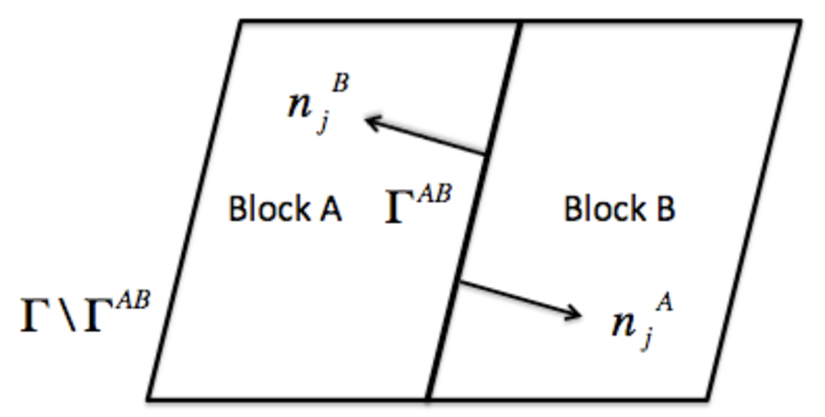
\includegraphics[height=1.5in]{images/twoBlockDiag.pdf}} 
 \caption{Two-block example with one common surface, $\Gamma_{AB}$.} 
 \label{domainAB} 
\end{figure}    

An interior penalty approach is constructed at each integration point at the 
exposed surface set. The numerical flux for a general scalar $\phi$ is constructed at the 
current integration point which is based on the current ($A$) and opposing ($B$) elemental 
contributions,

\begin{equation} 
        \int \hat Q^A dS = \int [\frac{(q_j^A n_j^A + q_j^B n_j^B)}{2}
				+ \lambda^A ( \phi^A - \phi^B) ]dS^A
        				+ \dot{m}^A \frac{(\phi^A + \phi^B)}{2},
\label{numericalFluxA}
\end{equation}
where $q_j^A$ and $q_j^B$ are the diffusive and convective fluxes computed using the current 
and opposing elements. The penalty coefficient $\lambda$ contains both advective and diffusive 
contributions averaged over the two elements. Above, the convection term is Galerkin approach,
however, upwinding has been implemented. Note that the lack of averaging the mass flow rate, 
$\dot{m}^A$ is somewhat arbitrary. The exact form of the mass flow rate is shown below and includes
full pressure stabilization terms.

Since this algorithm is a dual pass approach, a numerical flux can be written for the integration point on block $B$,

\begin{equation} 
        \int \hat Q^B dS = \int [\frac{(q_j^B n_j^B + q_j^A n_j^A)}{2} 
				+ \lambda^B ( \phi^B - \phi^A) ]dS^B
				+ \dot{m}^B \frac{(\phi^B + \phi^A)}{2}.
\label{numericalFluxB}
\end{equation}
Note that in each case, normals are outward facing. For low-order meshes with curved surface, faceting will occur.
In this case, the outward facing normals may not be (sign)-unity factors of each other. In this case, it
may be adventageous to define the opposing outward normal as, $n_j^B = -n_j^A$. 

Average fluxes are computed based on the current and opposing integration point locations. The 
appropriate DG terms are assembled as boundary conditions first with block $A$ integration 
points as $current$ (integrations points for block B are $opposing$) and then with block $B$ 
integration points as $current$ (surfaces for block A are, therefore, $opposing$). Figure~\ref{nonConformal} 
graphically demonstrates the procedure in which integration point values of the flux and penalty 
term are computed on the block $A$ surface and at the projected location of block $B$. 

\begin{figure}
\centering
  {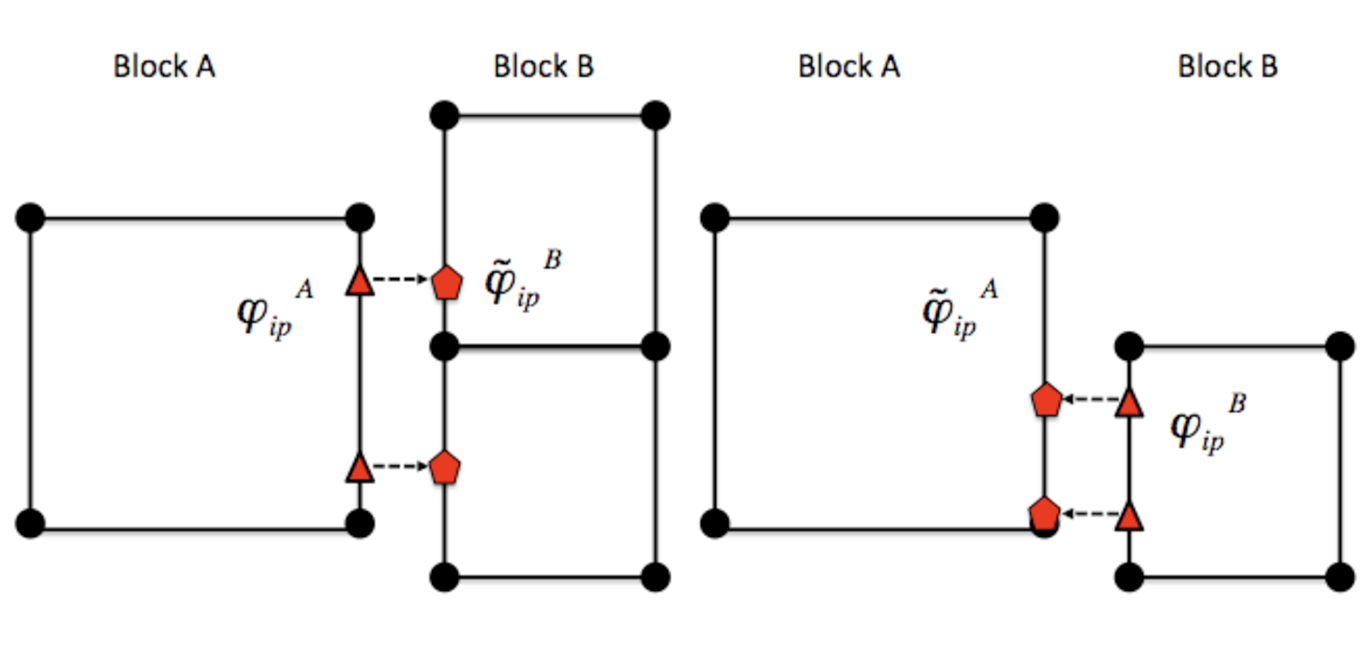
\includegraphics[height=1.5in]{images/contactSearchAndEval.pdf}}
  \vspace{0.25in}
  \caption{Description of the numerical flux calculation for the DG algorithm. The 
    value of fluxes and penalty values on the current block ($A$) and the opposing block ($B$) are used 
    for the calculation of numerical fluxes. $\tilde \varphi$ represents the projected value.}
  \label{nonConformal}
\end{figure}

A parallel search is conducted to project the current integration point location to the opposing element exposed face. 
The search, therefore, provides the isoparametric coordinates on the opposing element. Elemental shape functions 
and shape function derivatives are used to construct the numerical flux for both the edge- and element-based 
scheme. The location of the Gauss points on the current element are either the Gauss Labatto or Gauss Legendre 
locations (input file specification). For each equation (momentum, continuity, enthalpy, etc.) the numerical 
flux is computed at each exposed non-conformal surface.

The value of the penalty parameter, $\lambda$ contains advection and diffusion contributions. The current 
formulation defines this quantity as follows (here shown for current side $A$):

\begin{equation} 
        \lambda^A = \frac{(\Gamma^A / L^A + \Gamma^B / L^B )}{2} + |\dot{m}^A|,
\label{lamdbaA}
\end{equation}
where $\Gamma^k$ is the diffusive flux coefficient evaluated at current and opposing element location, respectively, 
and $L^k$ is an elemental length scale normal to the surface (again for current and opposing locations, $A$ and $B$). 
Again, the form of the penalty term is somewhat arbitrary in that the advection mass flow rate could have been upwinded 
or blended.

As noted, for most equations other than continuity and heat condition, the numerical flux includes advection and 
diffusion contributions. The diffusive contribution is easily provided using elemental shape function derivatives 
at the current and opposing surface. 

Above, special care is taken for the value of the mass flow rate at the non-conformal interface. Also,
note that the above written form does not upwind the advective flux, although the code allows for an upwinded 
approach. In general, the advective term contains contributions from both elements identified at the interface, 
specifically,

\begin{equation} 
        \dot {m}^A = \int [\frac{(\rho u_j^A + \tau G_j^A p -\tau \frac{\partial p^A}{\partial x_j}) 
        				       + (\rho u_j^B+ \tau G_j^B p -\tau \frac{\partial p^A}{\partial x_j})}{2}
				       + \lambda^A ( p^A - p^B)] dS^A.
\label{mdotA}
\end{equation}
The penalty coefficient for the mass flow rate at the non-conformal boundary points is again a function of the 
blended inverse length scale at the current and opposing element surface location. The form of the mass flow 
rate above provides the continuity contribution and the form of the mass flow rate used in the scalar non-conformal
flux contribution.

The full connectivity for element integration and opposing elements is within the linear 
system. As such, for sliding mesh configurations, the linear system connectivity graph changes each time step. Recent prototyping of 
the dG-based and the overset scheme has allowed this method to be used across both disparate low-order 
topologies (see Figure~\ref{dgMixMatch}).

\begin{figure}[h!tp]
\centering
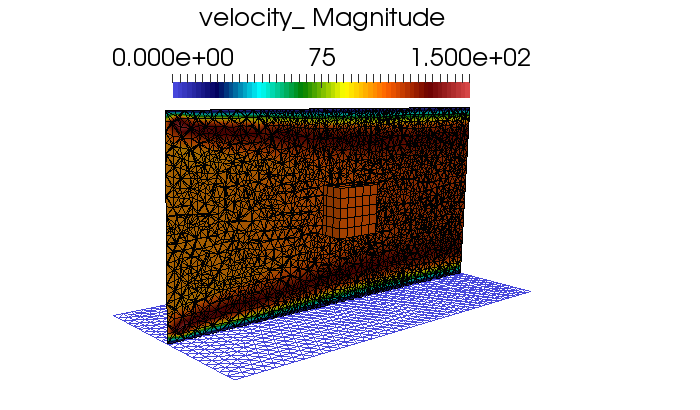
\includegraphics[clip,width=0.4\textwidth]{images/dgHex8Tet4Duct.png}
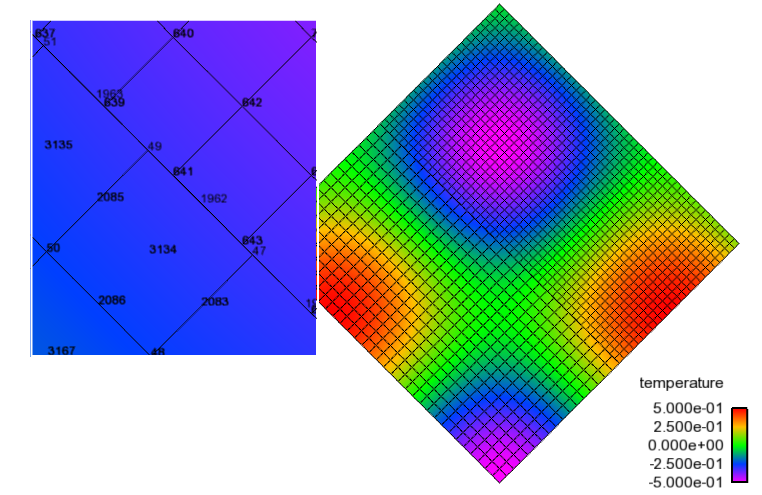
\includegraphics[clip,width=0.4\textwidth]{images/dgQuad4Quad9MMS.png}
\caption{Discontinuous Galerkin non-conformal interface mixed topology (left, hex8/tet4) and a low-order and high-order block interface 
(P=1 quad4 and P=2 quad9) for a MMS temperature solution (right). In the MMS image, the inset image is a close-up of the nodal 
Ids near the interface that highlights the quad4 and quad9 interface.}
\label{dgMixMatch}
\end{figure}


\section{Overset}
The overset descriptions begins with the basic background mesh (block 1) and
overset mesh (block 2) depicted in Figure~\ref{oversetBlockOneTwo}. Also
shown in this figure is the reduction outer surface of block 2 (light blue).
Elements within this reduced overset block will be determined by a parallel 
search. The collection of elements within this bounding box will be skinned 
to form a surface on which orphan nodes are placed. Elements within this volume
are set in a new internally managed inactive block. These mesh entities are 
fully removed from the overall matrix for each dof. Elements within this
volume are provided a masking integer element varibale of unity to select
out of the visualizattion tool. Therefore, orphan nodes live at the external 
boundary of block 2 and along the reduced surface. The parallel search provides
the mapping of orphan node and owning element from which the state can be 
constructured.

\begin{figure} [h]
\centerline{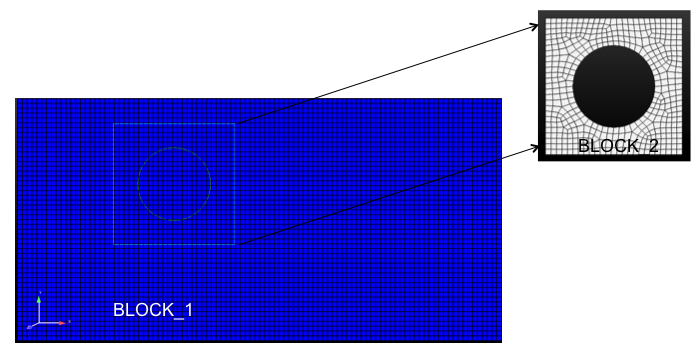
\includegraphics[height=3.0in]{images/oversetBlockOneTwo}}
\vspace{0.1in}
\caption{Two-block use case describing background mesh (block 1) and 
overset mesh (block 2).}
\label{oversetBlockOneTwo}
\end{figure}

After the full search and overset initialization, this simple example yields
the original block 1 and 2, the newly created inactive block 3, the original
surface of the overset mesh and the new skinned surface (101) of the innactive
block (Figure~\ref{oversetBlockOneTwoCut}.

\begin{figure} [h]
\centerline{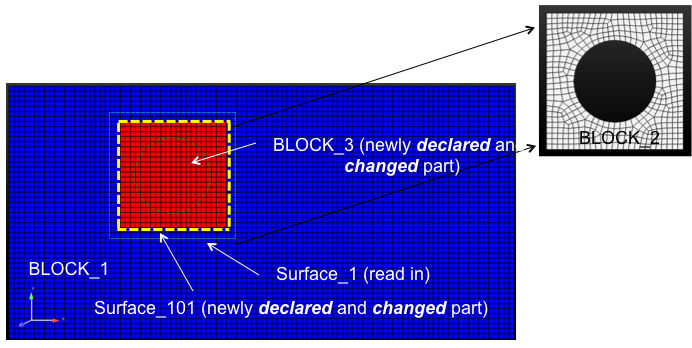
\includegraphics[height=3.0in]{images/oversetBlockOneTwoCut}}
\vspace{0.1in}
\caption{Three-block and two surface, post over set initialization.}
\label{oversetBlockOneTwoCut}
\end{figure}

A simple heat conduction example is provided in Figure~\ref{oversetHC} where
the circular boundary is set at a temperature of 500 with all external 
boundaries set to adiabatic.

\begin{figure} [h]
\centerline{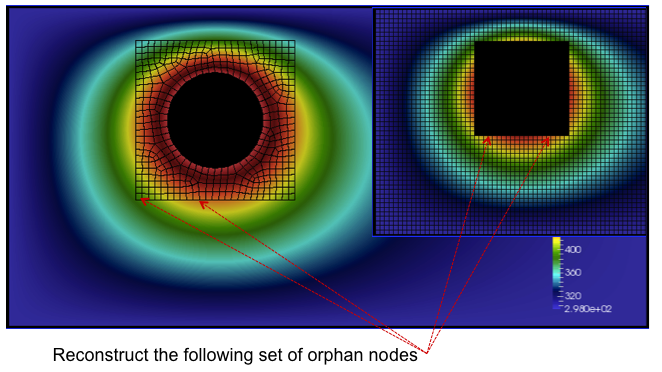
\includegraphics[height=3.0in]{images/oversetHC}}
\vspace{0.1in}
\caption{A simple heat conduction example providing the overset mesh and
donor orphan nodes.}
\label{oversetHC}
\end{figure}

As noted before, every orphan node lies within an owning element. Sufficient
overlap is required to make the system well posed. A fully implicit procedure
is provided by writing the orphan node value as a linear constraint of the
owning element (Figure~\ref{orphanNodes}).

\begin{figure} [h]
\centerline{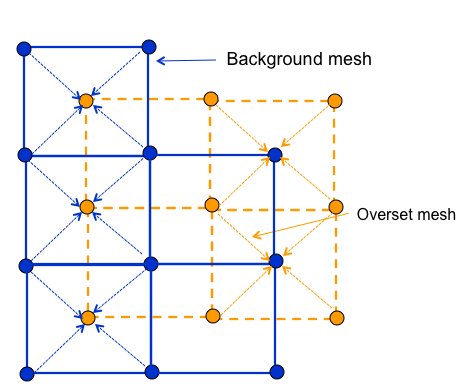
\includegraphics[height=3.0in]{images/oversetNodes}}
\vspace{0.1in}
\caption{Orphan nodes for background and overset mesh for which a fully 
implicit constraint equation is written.}
\label{oversetNodes}
\end{figure}

For completeness, the constraint equation for any dof $\phi^o$ is simply,
\begin{equation}
  \phi^o - \sum N_k \phi_k = 0.
\label{constraint}
\end{equation}
As noted, full sensitivities are provided in the linear system by constructing
a row entry with the columns of the nodes within the owning element and the
orphan node itself.

Finally, a mixed hex/tet mesh configuration example (overset mesh is tet 
while background is hex) is provided in Figure~\ref{oversetSphere}.

\begin{figure} [h]
\centerline{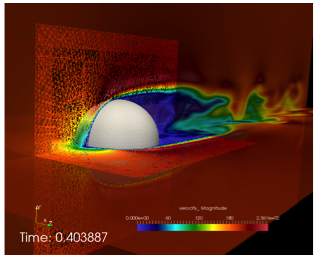
\includegraphics[height=3.0in]{images/oversetSphere}}
\vspace{0.1in}
\caption{Flow past a three-dimensional sphere using a hybrid topology 
(hex/tet) mesh configuration.}
\label{oversetHC}
\end{figure}

\subsection{Future Capabilities}

The overset capability has not been modified to work with generalized mesh
motion. Moreover, search and cutting is reserved for simple squares and 
rectangular overset meshes.




\section{Property Evaluations}
Property specification is provided in the material model section of the input file. 
Unity Lewis number assumptions for diffusive flux coefficients for mass fraction and enthalpy are assumed.

\subsubsection{Density}
At present, property evaluation for density is given by constant, single mixture fraction-based, HDF5 tables, or ideal gas. For ideal gas, we support a non-isothermal, non-uniform and even an acoustically compressible form.

\subsubsection{Viscosity}
Property evaluation for viscosity is given by constant, single mixture fraction-based, simple tables
or Sutherland's three coefficient as a function of temperature. When mixtures are used, either by reference or 
species transport, only a mass fraction-weighed approach is used.

\subsubsection{Specific Heat}
Property evaluation for specific heat is either constant of two-band standard NASA polynomials; again species composition weighting are used (either transported or reference).

\subsubsection{Lame Properties}
Lame constants are either of type constant or for use in mesh motion/smoothing geometric whereby
the values are inversely proportional to the dual volume.



\section{Coupling Approach}
\input{couplingApproach}

\section{Time discretization}
\input{timeDiscretization}

\section{Multi-Physics}
\input{multiPhysics}

\section{Topological Support}
The currently supported elements are as follows: hex, tet, pyramid, wedge, quad, and tri. 
In general, hybrid meshes are fully supported for the edge-based scheme. For CVFEM,
hybrid meshes are also supported, however, wedge and pyramid elements are not permitted
at exposed open or symmetry boundaries. The remedy to the CVFEM constraint is to
simply implement the exposed face gradient operators.


\section{Adaptivity}
Adaptivity is supported through usage of the Percept module. However, this code base has not yet
been deployed to the open sector. As such, ifdef guards are placed within the code base. A variety of 
choices exist for the manner by which hanging nodes are removed in a vertex-centered code base.

A typical h-adapted patch of elements
is shown in Figure~\ref{hadapt-convol}.  The ``hanging nodes"
do not have control volumes associated with them.  Rather,
they are constrained to be a linear combination of the
two parent edge nodes.  There is no element assembly procedure 
to compute fluxes for the ``hanging sub-faces" associated with the hanging 
nodes that occur along the parent-child element boundary.

\begin{figure}[h]
  \centerline{\includegraphics[width=5.5in]{images/hadapt.pdf}}
  \vspace{0.25in}
  \caption{Control volume definition on an h-adapted mesh
           with hanging nodes. (Four-patch of parent elements 
           with refinement in bottom-right element.) }
  \label{hadapt-convol}
\end{figure}

\noindent
In general, for a vertex-centered scheme, the h-adaptive scheme is driven at the element level.
Refinement occurs within the element and the topology of refined elements is the same as the parent element. 

Aftosmis~\cite{Aftosmis:94} describes a vertex-centered
finite-volume scheme on unstructured Cartesian meshes.
A transitional set of control volumes are formed about
the hanging nodes, shown in Figure~\ref{aftosmis-convol}.  
on unstructured meshes. This approach would require a
series of specialized master elements to deal with the
different transition possibilities.

\begin{figure}[h]
  \centerline{\includegraphics[width=3.5in]{images/hadapt2.pdf}}
  \vspace{0.25in}
  \caption{Control volume definition on an h-adapted mesh
           with transition control volumes about the
           hanging nodes. (Four-patch of parent elements 
           with refinement in bottom-right element.) }
  \label{aftosmis-convol}
\end{figure}

Kallinderis~\cite{Kallinderis:89} describes a vertex-centered
finite-volume scheme on unstructured quad meshes.  Hanging
nodes are treated with a constraint condition.  The flux
construction for a node on a refinement boundary is based
on the unrefined parent elements, leading to a 
non-conservative scheme.

Kallinderis~\cite{kallinderis:93} also describes a vertex-centered
finite-volume scheme on unstructured tetrahedral meshes.  Hanging
nodes are removed by splitting the elements on the ``unrefined"
side of the refinement boundary. Mavriplis~\cite{Mavriplis:00} uses a similar 
technique, however, extends it to a general set of heterogeneous elements,
shown in Figure~\ref{kallin-convol}.

\begin{figure}[h]
  \centerline{\includegraphics[width=3.5in]{images/hadapt3.pdf}}
  \vspace{0.25in}
  \caption{Control volume definition on a heterogeneous
           h-adapted mesh with no hanging nodes.
           (Four-patch of parent elements 
           with refinement in bottom-right element
           and splitting in adjacent parent elements.) }
  \label{kallin-convol}
\end{figure}

The future deployment of Percept will use the procedure of Mavriplis whereby hanging 
nodes are removed by neighbor topological changes. A variety of error indicators exists 
and a prototyped error transport equation appraoch for the one-equation $k^{sgs}$ model 
has been tested for classic jet-in-crossflow configurations.

\subsection{Prolongation and Restriction}

Nodal variables are interpolated between levels of the
h-adapted mesh hierarchy using the traditional prolongation
and restriction operators defined over an element.  The
prolongation operation is used to compute values for new
nodes that arise from element sub-division.  The parent element
shape functions are used to interpolate values from the parent
nodes to the sub-divided nodes.

Prolongation and restriction operators for element variables and 
face variables are required to maintain mass flow rates that
satisfy continuity. When adaptivity takes place, a code option
to reconstruct the mass flow rates must be used. Whether or not
a Poisson system must be created has been explored. More work is 
required to understand the nuances associated with prolongation, 
specifically with respect to possible dispersion errors.


\section{Code Abstractions}
The Nalu code base is a c++ code-base that significantly leverages
the Sierra Toolkit and Trilinos infrastructure. This section is designed to
provide a high level overview of the underlying abstractions that the 
code base exercises. For more detailed code information, the developer is referred to
the Trilinos project (github.com). In
the sections that follow, only a high level overview is provided. 

The developer might also find useful examples in the NaluUnit github repository
as it contains a number of specialized implementations that are very small in nature.
In fact, the Nalu code base emerged as a small testbed unit test to evaluate the STK
infrastructure. Interestingly, the first 
``algorithm'' implementation was a simple $L_2$ projected nodal gradient. This effort 
involved reading in a mesh, registering a nodal (vector) field, iterating elements 
and exposed surfaces to assemble the projected nodal gradient to the nodes of the mesh
(in parallel). When evaluating kokkos, this algorithm was also used to learn about 
the parallel NGP abstraction provided.

\subsection{Sierra Toolkit Abstractions}
Consider a typical mesh that consists of nodes, sides of elements and elements.
Such a mesh, when using the Exodus standard, will liekly be represented by a 
collection of ``element blocks'', ``sidesets'' and, possibly, ``nodesets''. The 
definition of the mesh (generated by the user through commercial meshing packages such as
pointwise or ICM-CFD) will provide the required spatial definitions of the volume physics 
and the required boundary conditions.

An element block is a homegeneous collection of elements of the same
underlying topology, e.g., HEXAHEDRAL-8. A sideset is a set of exposed element faces
on which a boundary condition is to be applied. Finally, a nodeset is a collection of 
nodes. In general, nodesets are possibly output entities as the code does not exercise
enforcing physics or boundary conditions on nodesets. Although Nalu supports an edge-based
scheme, an edge, which is an entity connecting two nodes, is not part of the Exodus standard
and must be generated within the STK infrastructure. Therefore, a particular discretization
choice may require $stk::mesh::Entity$ types of element, face (or side), edge and node.

Once the mesh is read in, a variety of routine operations are generally required. For example,
a low-Mach physics equation set may want to be applied to $block_1$ while inflow, open, symmetry, 
periodic and wall boundary conditions can be applied to a variety of sidesets. For example, 
$surface_1$ might be of an ``inflow'' type. Therefore, the high level set of requirements on a mesh 
infrastructure might be to allow one to iterate parts of the mesh and, in the end, assemble
a quantity to a nodal or elemental field. 

\subsubsection{Meta and Bulk Data}
Meta and Bulk data are simply STK containers. MetaData is used to extract parts, 
extract ownership status, determine the side rank, field declaration, etc. 
BulkData is used to extract buckets, extract upward and downward connectivities 
and determine node count for a given entity.

\subsubsection{Parallel Rules}
In STK, elements are locally owned by a single rank. Elements may be ghosted to other parallel ranks
through STK custom ghosting. Exposed faces are locally owned by the lower parallel rank. Nodes
are also locally owned by the lower parallel rank and can also be shared by all parallel ranks touching
them. Edges and internal faces (element:face:element connectivity) have the same rule of locally 
owned/shared and can also be ghosted. Again, edges and internal faces must be created by existing
STK methods should the physics algorithm require them. In Nalu, the choice of element-based 
or edge-based is determined within the input file.

\subsubsection{Connectivity}
In an unstructured mesh, connectivity must be built from the mesh and can not be assumed to 
follow an assumed ``i-j-k'' data layout, i.e., structured. In general, one speaks of downward and upward 
relationships between the underlying entities. For example, if one has a particular element, one might
like to extract all of the nodes connected to the element. Likewise, this represents a common opporation
for faces and edges. Such examples are those in which downward relationships are required. 
However, one might also have a node and want to extract all of the connected elements to this 
node (consider some sort of patch recovery algorithm). STK provides the ability to extract 
such connectivities. In general, full downward and upward connectivites are created.

For example, consider an example in which one has a pointer to an element and wants to 
extract the nodes of this element. At this point, the developer has not been exposed to 
abstractions such as buckets, selectors, etc. As such, this is a very high level overview
with more details to come in subsequent sections. Therefore, the scope below is to assume that
from an element-k of a ``bucket'', b[k] (which is a collection of homegeneous RANK-ed entities) 
we will extract the nodes of this element using the STK bulk data.

\begin{lstlisting}

// extract element from this bucket
stk::mesh::Entity elem = b[k];

// extract node relationship from bulk data
stk::mesh::Entity const * node_rels = bulkData_.begin_nodes(elem);
int num_nodes = bulkData_.num_nodes(elem);

// iterate nodes
for ( int ni = 0; ni < num_nodes; ++ni ) {
  stk::mesh::Entity node = node_rels[ni];
  
  // set connected nodes
  connected_nodes[ni] = node;
  
  // gather some data, e.g., density at state Np1, into a local workset pointer
  p_density[ni] = *stk::mesh::field_data(densityNp1, node );
}

\end{lstlisting}

\subsubsection{Parts}
As noted before, a $stk::mesh::Part$ is simply an abstraction that describes a 
set of mesh entities. If one has the name of the part from the mesh data base,
one may extract the part. Once the part is in hand, one may iterate the underlying set of
entities, walk relations, assemble data, etc.

The following example simply extracts a part for each vector of names that lives in
the vector $targetNames$ and provides this part to all of the underlying equations
that have been created for purposes of nodal field registration. Parts of the mesh
that are not included within the $targetNames$ vector would not be included in the 
field registration and, as such, if this mising part was used to extract the data, an 
error would occur.

\begin{lstlisting}

for ( size_t itarget = 0; itarget < targetNames.size(); ++itarget ) {
  stk::mesh::Part *targetPart = metaData_.get_part(targetNames[itarget]);

  // check for a good part
  if ( NULL == targetPart ) {
    throw std::runtime_error("Trouble with part " + targetNames[itarget]);
  }
  else {
    EquationSystemVector::iterator ii;
    for( ii=equationSystemVector_.begin(); ii!=equationSystemVector_.end(); ++ii )
    (*ii)->register_nodal_fields(targetPart);
  }
}

\end{lstlisting}

\subsubsection{Selectors}
In order to arrive at the percise parts of the mesh and entities on which one desires
to operate, one needs to ``select'' what is useful. The STK selector infrastructure provides this.

In the following example, it is desired to obtain a selector that containst all of the parts of 
interest to a physics algorithm that are locally owned and active.

\begin{lstlisting}

// define the selector; locally owned, the parts I have served up and active
stk::mesh::Selector s_locally_owned_union = metaData_.locally_owned_part()
  & stk::mesh::selectUnion(partVec_) 
  & !(realm_.get_inactive_selector());

\end{lstlisting}

\subsubsection{Buckets}
Once a selector is defined (as above) an abstraction to provide access to the type of 
data can be defined. In STK, the mechanism to iterate entities on the mesh is through the 
bucket interface. A bucket is a homegenous collection of $stk::mesh::Entity$.

In the below example, the selector is used to define the bucket of entities that are provided
to the developer.

\begin{lstlisting}
// given the defined selector, extract the buckets of type ``element''
stk::mesh::BucketVector const& elem_buckets 
  = bulkData_.get_buckets( stk::topology::ELEMENT_RANK, 
                           s_locally_owned_union );

// loop over the vector of buckets 
for ( stk::mesh::BucketVector::const_iterator ib = elem_buckets.begin();
      ib != elem_buckets.end() ; ++ib ) {
  stk::mesh::Bucket & b = **ib ;
  const stk::mesh::Bucket::size_type length   = b.size();

  // extract master element (homogeneous over buckets)
  MasterElement *meSCS = realm_.get_surface_master_element(b.topology());
  
  for ( stk::mesh::Bucket::size_type k = 0 ; k < length ; ++k ) {
    
    // extract element from this bucket
    stk::mesh::Entity elem = b[k];
    
    // etc...
  }
}

\end{lstlisting}

The look-and-feel for nodes, edges, face/sides is the same, e.g.,

\begin{description}
\item[$\bullet$ for nodes:]
\end{description}

\begin{lstlisting}
// given the defined selector, extract the buckets of type ``node''
stk::mesh::BucketVector const& node_buckets 
  = bulkData_.get_buckets( stk::topology::NODE_RANK, 
                           s_locally_owned_union );

// loop over the vector of buckets 
\end{lstlisting}

\begin{description}
\item[$\bullet$ for edges:]
\end{description}

\begin{lstlisting}
// given the defined selector, extract the buckets of type ``edge''
stk::mesh::BucketVector const& edge_buckets 
  = bulkData_.get_buckets( stk::topology::EDGE_RANK, 
                           s_locally_owned_union );

// loop over the vector of buckets 
\end{lstlisting}


\begin{description}
\item[$\bullet$ for faces/sides:]
\end{description}

\begin{lstlisting}
// given the defined selector, extract the buckets of type ``face/side''
stk::mesh::BucketVector const& face_buckets 
  = bulkData_.get_buckets( metaData_.side_rank(), 
                           s_locally_owned_union );

// loop over the vector of buckets 
\end{lstlisting}


\subsubsection{Field Data Registration}
Given a part, we would like to declare the field and put the field on the part of interest.
The developer can register fields of type elemental, nodal, face and edge of desired size. 

\begin{description}
\item[$\bullet$ nodal field registration:]
\end{description}

\begin{lstlisting}
void
LowMachEquationSystem::register_nodal_fields(
  stk::mesh::Part *part)
{
  // how many states? BDF2 requires Np1, N and Nm1
  const int numStates = realm_.number_of_states();

  // declare it
  density_ 
    =  &(metaData_.declare_field<ScalarFieldType>(stk::topology::NODE_RANK, 
                                                 "density", numStates));

  // put it on this part
  stk::mesh::put_field(*density_, *part);
}
\end{lstlisting}

\begin{description}
\item[$\bullet$ edge field registration:]
\end{description}

\begin{lstlisting}
void
LowMachEquationSystem::register_edge_fields(
  stk::mesh::Part *part)
{
  const int nDim = metaData_.spatial_dimension();
  edgeAreaVec_ 
    = &(metaData_.declare_field<VectorFieldType>(stk::topology::EDGE_RANK, 
                                                "edge_area_vector"));
  stk::mesh::put_field(*edgeAreaVec_, *part, nDim);
}
\end{lstlisting}

\begin{description}
\item[$\bullet$ side/face field registration:]
\end{description}

\begin{lstlisting}
void
MomentumEquationSystem::register_wall_bc(
  stk::mesh::Part *part,
  const stk::topology &theTopo,
  const WallBoundaryConditionData &wallBCData)
{
  // Dirichlet or wall function bc
  if ( wallFunctionApproach ) {
    stk::topology::rank_t sideRank 
      = static_cast<stk::topology::rank_t>(metaData_.side_rank());
    GenericFieldType *wallFrictionVelocityBip 
      =  &(metaData_.declare_field<GenericFieldType>
          (sideRank, "wall_friction_velocity_bip"));
    stk::mesh::put_field(*wallFrictionVelocityBip, *part, numIp);
  }
}
\end{lstlisting}

\subsubsection{Field Data Access}
Once we have the field registered and put on a part of the mesh, we can extract the field
data anytime that we have the entity in hand. In the example below, we extract nodal field
data and load a workset field.

To obtain a pointer for a field that was put on a node, edge face/side or element field, 
the string name used for declaration is used in addition to the field template type,

\begin{lstlisting}
VectorFieldType *velocityRTM 
  = metaData_.get_field<VectorFieldType>(stk::topology::NODE_RANK, 
                                        "velocity");
ScalarFieldType *density 
  = metaData_.get_field<ScalarFieldType>(stk::topology::NODE_RANK, 
                                        "density");}

VectorFieldType *edgeAreaVec 
  = metaData_.get_field<VectorFieldType>(stk::topology::EDGE_RANK, 
                                        "edge_area_vector");

GenericFieldType  *massFlowRate
  = metaData_.get_field<GenericFieldType>(stk::topology::ELEMENT_RANK, 
                                         "mass_flow_rate_scs");

GenericFieldType *wallFrictionVelocityBip_ 
  = metaData_.get_field<GenericFieldType>(metaData_.side_rank(), 
                                         "wall_friction_velocity_bip");
\end{lstlisting}

\subsubsection{State}
For fields that require state, the field should have been declared with the 
proper number of states (see field declaration section). Once the field pointer is 
in hand, the specific field with state is easily extracted,

\begin{lstlisting}
ScalarFieldType *density 
  = metaData_.get_field<ScalarFieldType>(stk::topology::NODE_RANK, 
                                        "density");
densityNm1_ = &(density->field_of_state(stk::mesh::StateNM1));
densityN_ = &(density->field_of_state(stk::mesh::StateN));
densityNp1_ = &(density->field_of_state(stk::mesh::StateNP1));
\end{lstlisting}

With the field pointer already in hand, obtaining the particular data
is field the field data method.

\begin{description}
\item[$\bullet$ nodal field data access:]
\end{description}

\begin{lstlisting}
// gather some data (density at state Np1) into a local workset pointer
p_density[ni] = *stk::mesh::field_data(densityNp1, node );
\end{lstlisting}

\begin{description}
\item[$\bullet$ edge field data access:] (from an edge bucket loop with the same selector as defined above)
\end{description}

\begin{lstlisting}
stk::mesh::BucketVector const& edge_buckets 
  = bulkData_.get_buckets( stk::topology::EDGE_RANK, s_locally_owned_union );
for ( stk::mesh::BucketVector::const_iterator ib = edge_buckets.begin();
      ib != edge_buckets.end() ; ++ib ) {
  stk::mesh::Bucket & b = **ib ;
  const stk::mesh::Bucket::size_type length   = b.size();

  // pointer to edge area vector and mdot (all of the buckets)
  const double * av = stk::mesh::field_data(*edgeAreaVec_, b);
  const double * mdot = stk::mesh::field_data(*massFlowRate_, b);
  
  for ( stk::mesh::Bucket::size_type k = 0 ; k < length ; ++k ) {
    // copy edge area vector to a pointer
    for ( int j = 0; j < nDim; ++j )
      p_areaVec[j] = av[k*nDim+j];
     
    // save off mass flow rate for this edge
    const double tmdot = mdot[k];
  }
}
\end{lstlisting}

\subsection{High Level Nalu Abstractions}

\subsubsection{Realm}
A realm holds a particlular physics set, e.g., low-Mach fluids. Realms are coupled
loosely through a transfer operation. For example, one might have a turbulent 
fluids realm, a thermal heat conduction realm and a PMR realm. The realm also 
holds a BulkData and MetaData since a realm requires fields and parts to solve
the desired physics set.

\subsubsection{EquationSystem}
An equation system holds the set of PDEs of interest. As Nalu uses a pressure projection
scheme with split PDE systems, the pre-defined systems are, LowMach, MixtureFraction,
Enthalpy, TurbKineticEnergy, etc. New monolithic equation system can be easily created and 
plugged into the set of all equation systems.

In general, the creation of each equation system is of arbitrary order, however, in some cases
fields required for MixtureFraction, e.g., $mass_flow_rate$ might have only been registered
on the low-Mach equaiton system. As such, if MixtureFraction is created before LowMachEOS,
an error might be noted. This can be easily resolved by cleaning the code base such that
each equation system is ``autonomous''.

Each equation system has a set of virtual methods expected to be implemented. These include, however,
are not limited to registration of nodal fields, edge fields, boundary conditions of fixed
type, e.g., wall, inflow, symmetry, etc.



\bibliographystyle{unsrt}
\bibliography{references}

\end{document} 
